\documentclass[Orbiter User Manual.tex]{subfiles} 
\begin{document}

\section{Included spacecraft types}
Orbiter comes with a range of diverse spacecraft types to explore different aspects of space flight. This includes fictional spacecraft such as the Delta-glider and Shuttle-A which relax a few specifications beyond current limits (in particular in terms of fuel efficiency and structural strength) to allow flights across the solar system, recreations of real vessels such as the Space Shuttle with narrow error margins that require precise flight plans, to novel concepts such as solar sails.\\
The spacecraft included in the basic Orbiter distribution will get you started, but many more can be downloaded as add-ons. See the Orbiter web page for a list of add-on repositories.


\subsection{Delta-glider}

\begin{figure}[H]
  \centering
  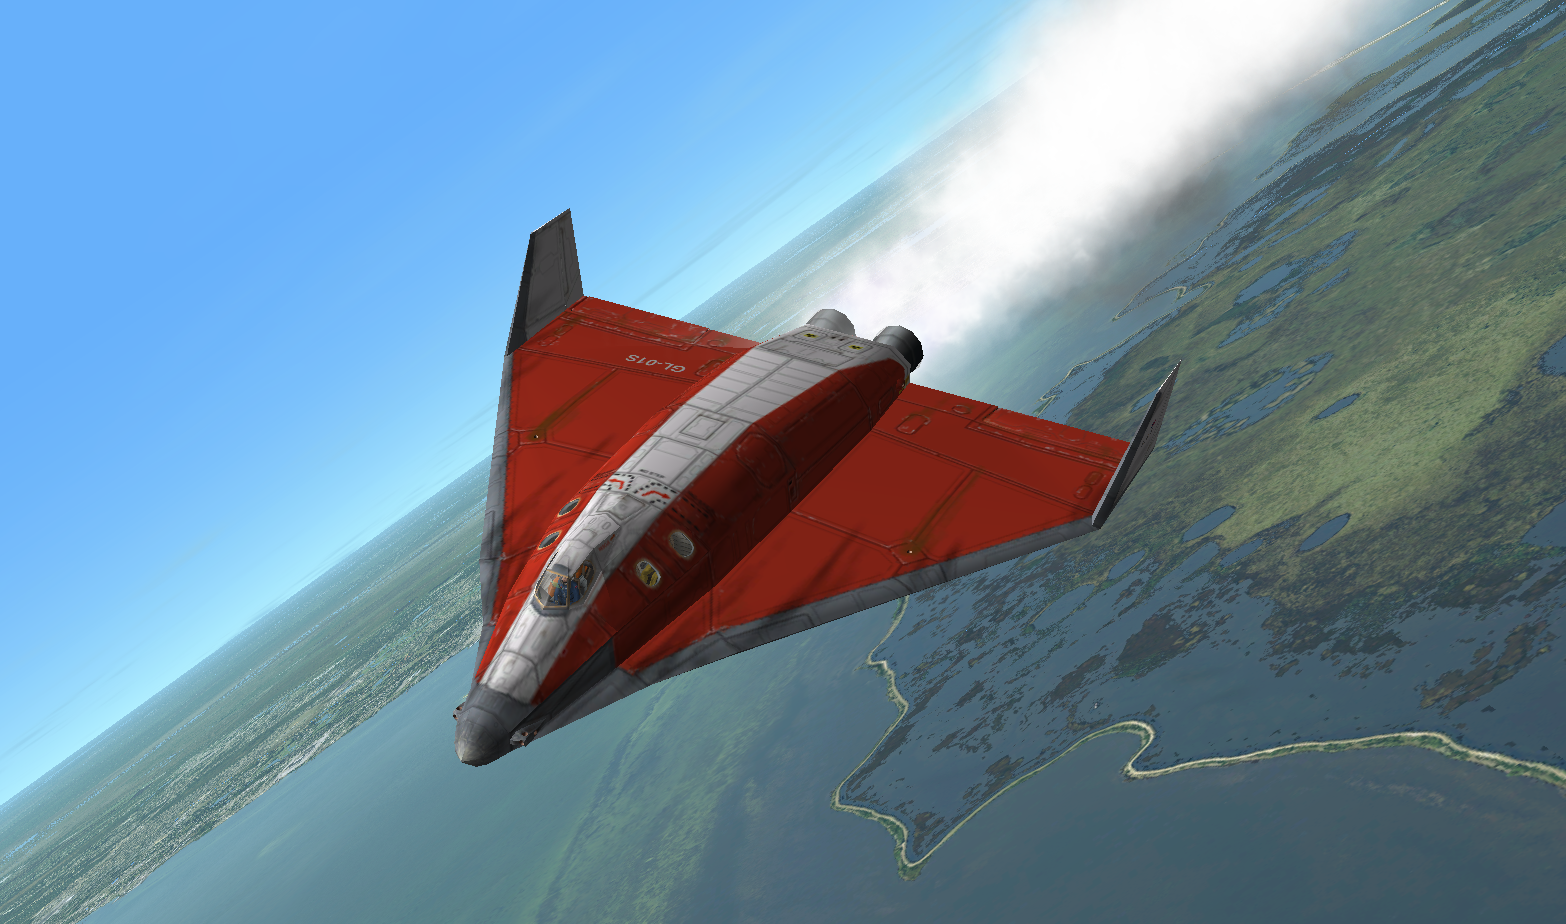
\includegraphics[width=0.75\hsize]{dg.png}
  \caption{Delta-glider model and textures by Roger "Frying Tiger" Long. Instrument panels by Martin Schweiger.}
\end{figure}

\noindent
The Delta-glider (DG) is the ideal ship for the novice pilot to get space-borne. Its futuristic design concept, high thrust and extremely low fuel consumption make it easy to achieve orbit, and it can even be used for interplanetary travel. The winged body provides aircraft-like handling in the lower atmosphere, while the vertically mounted hover thrusters allow vertical lift-offs and landings independent of atmospheric conditions and runways.\\
Two versions are available: The standard DG is equipped with main, retro and hover engines. The scramjet version (DG-S) has in addition two air-breathing scramjet engines fitted, which can be used during supersonic atmospheric flight. The scramjets have an operational airspeed range of Mach 3-8.\\
The DG supports 2-D instrument panels and a virtual cockpit in addition to the standard "glass cockpit" camera mode.\\
The glider comes with operational landing gear, nose cone docking port, airlock door, deployable radiator and animated aerodynamic control surfaces.


\subsubsection{Cockpit camera modes}
Apart from the generic "glass cockpit" camera mode which supports a head-up display (HUD), up to two multi-functional displays (MFD) and some of the most essential control and display components, the DG also provides a set of 2-D instrument panels, and a virtual 3-D cockpit (VC), all of which can be operated with the mouse. You can switch between the different cockpit modes by pressing \keystroke{F8}.

\paragraph{2-D instrument panels}
The glider supports a 2-D panel mode consisting of main and overhead instrument panel which can be selected with \Ctrl\UArrow and \Ctrl\DArrow. The panels can be scrolled up and down with \UArrow and \DArrow. Active panel elements, such as buttons, switches and dials can be operated with the left mouse button. Pressing the right mouse button and dragging the mouse rotates the camera. The camera can be reset to the default forward direction with the \Home key.

\begin{figure}[H]
  \centering
  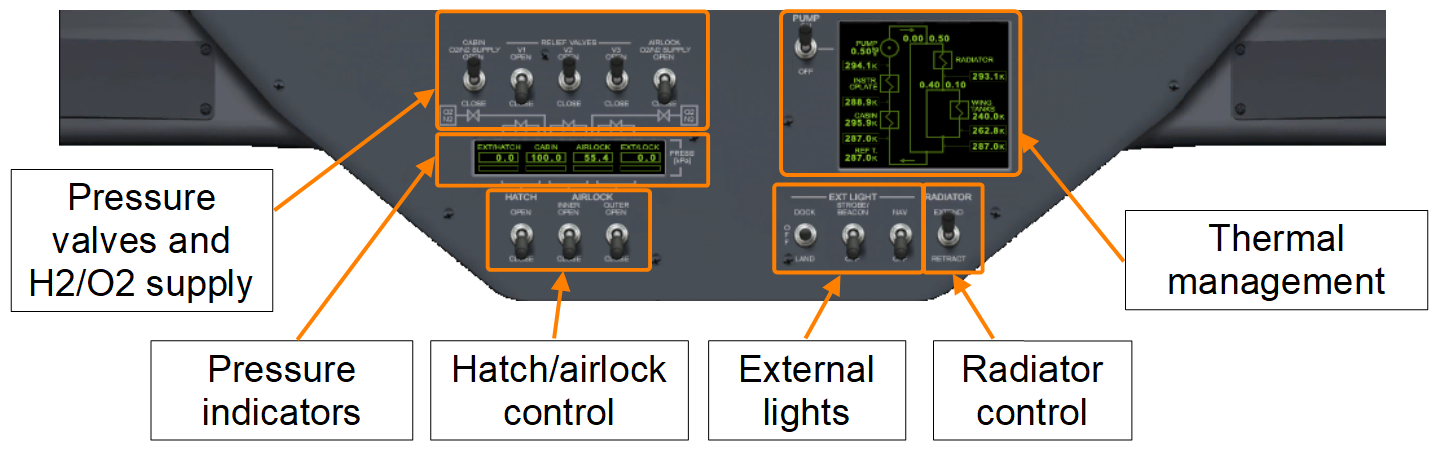
\includegraphics[width=\hsize]{dg_panel1.png}
%\end{figure}
%\begin{figure}[H]
%  \centering
  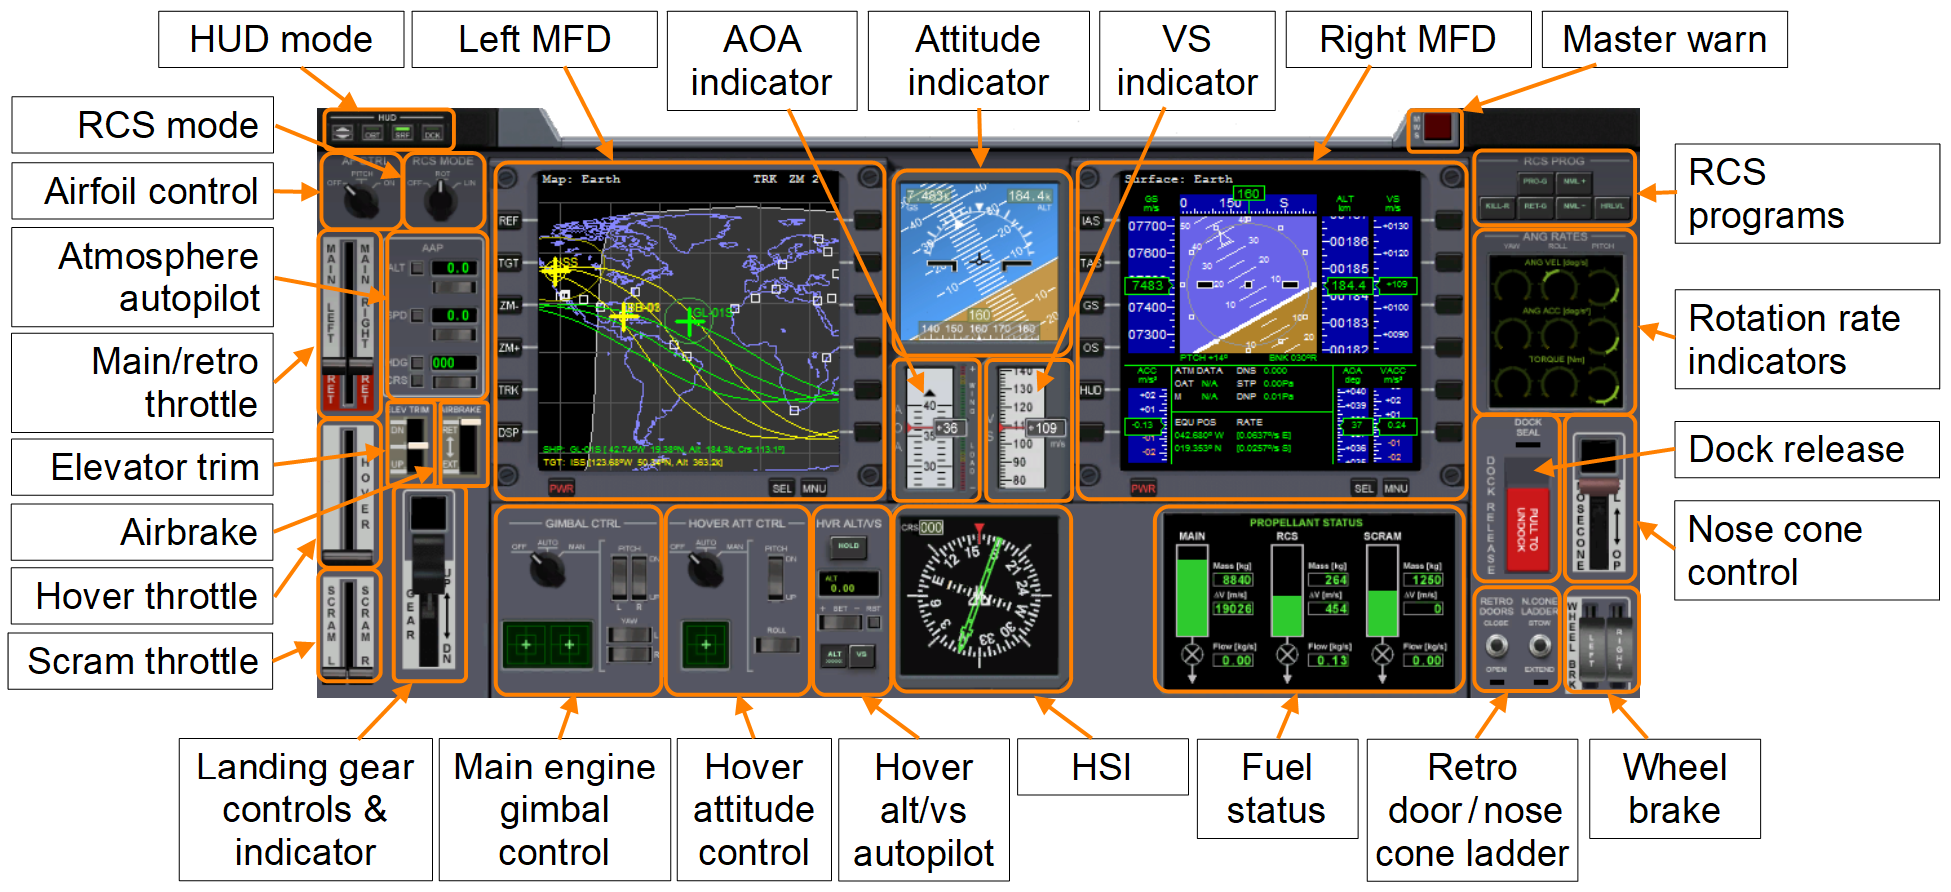
\includegraphics[width=\hsize]{dg_panel0.png}
  \caption{Delta-glider 2D overhead and main panels.}
\end{figure}

\paragraph{Virtual cockpit}
The Delta-glider provides a 3-D virtual cockpit (VC) mode in addition to the 2-D panel mode. The VC puts you in the pilot's seat, with the head-up display in front of you, and all avionics controls and displays within easy reach. You can operate switches and levers with the mouse. Look around you by pressing the right mouse button and dragging the mouse, by using \Alt\UArrow\DArrow\LArrow\RArrow, or with the coolie hat on your joystick. You can also lean left, right and forward with \Ctrl\Alt\UArrow\DArrow\LArrow\RArrow, to get a better view of your surroundings.\\
The field of view can be adjusted with the mouse wheel or with the \keystroke{Z} and \keystroke{X} buttons. This is useful for zooming in on specific instruments. Cockpit and external field of view settings are adjusted independently.

\begin{figure}[H]
  \centering
  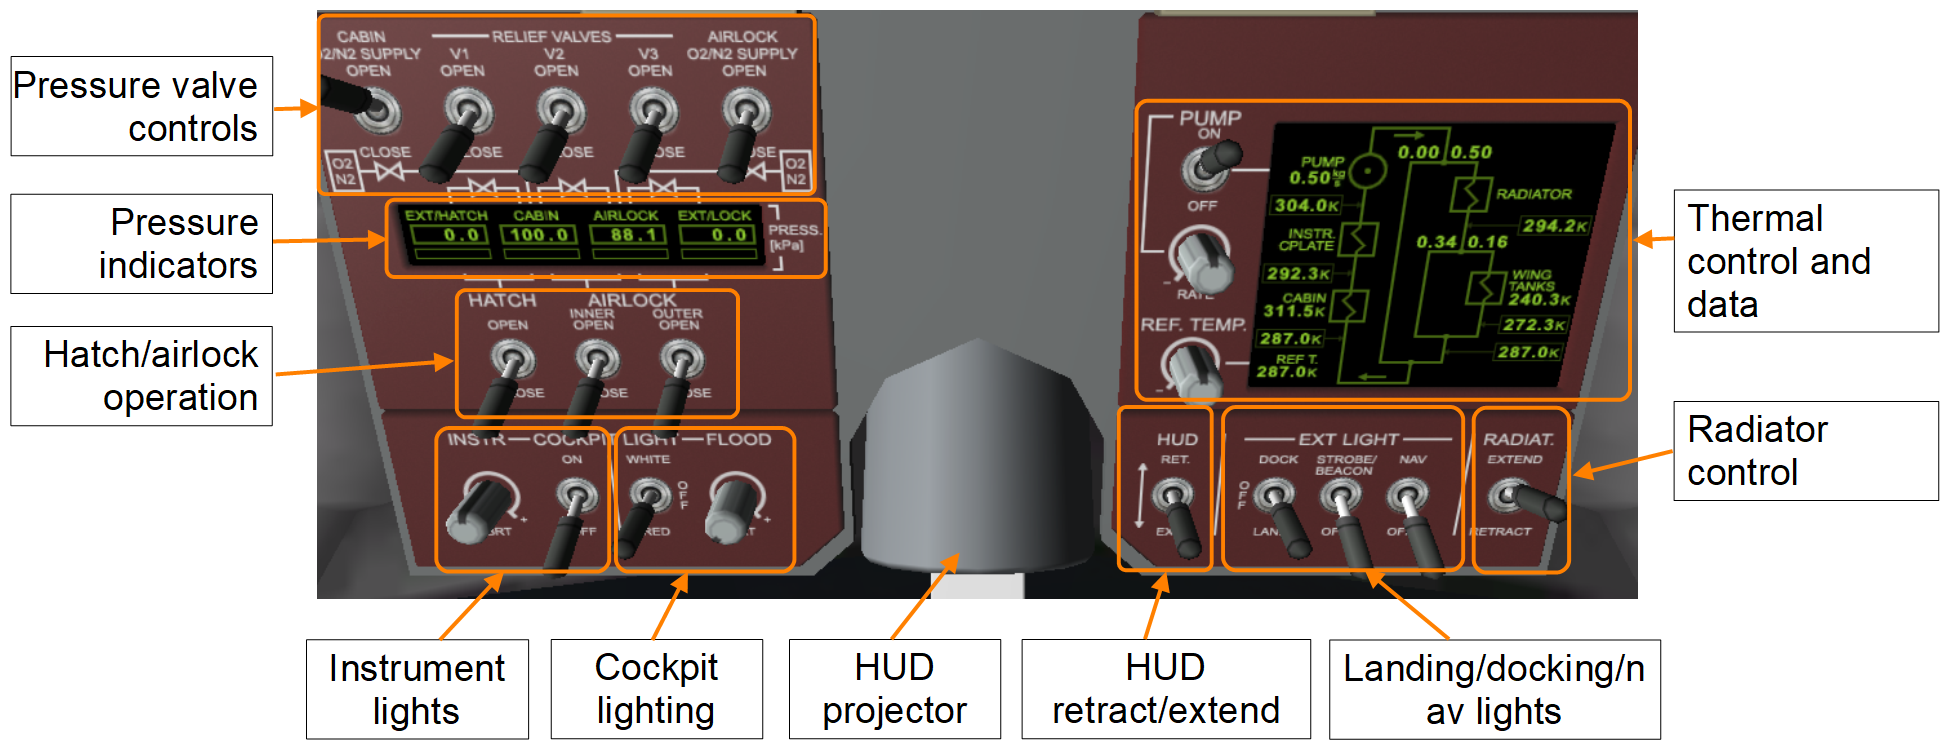
\includegraphics[width=\hsize]{dg_VC1.png}
%\end{figure}
%\begin{figure}[H]
%  \centering
  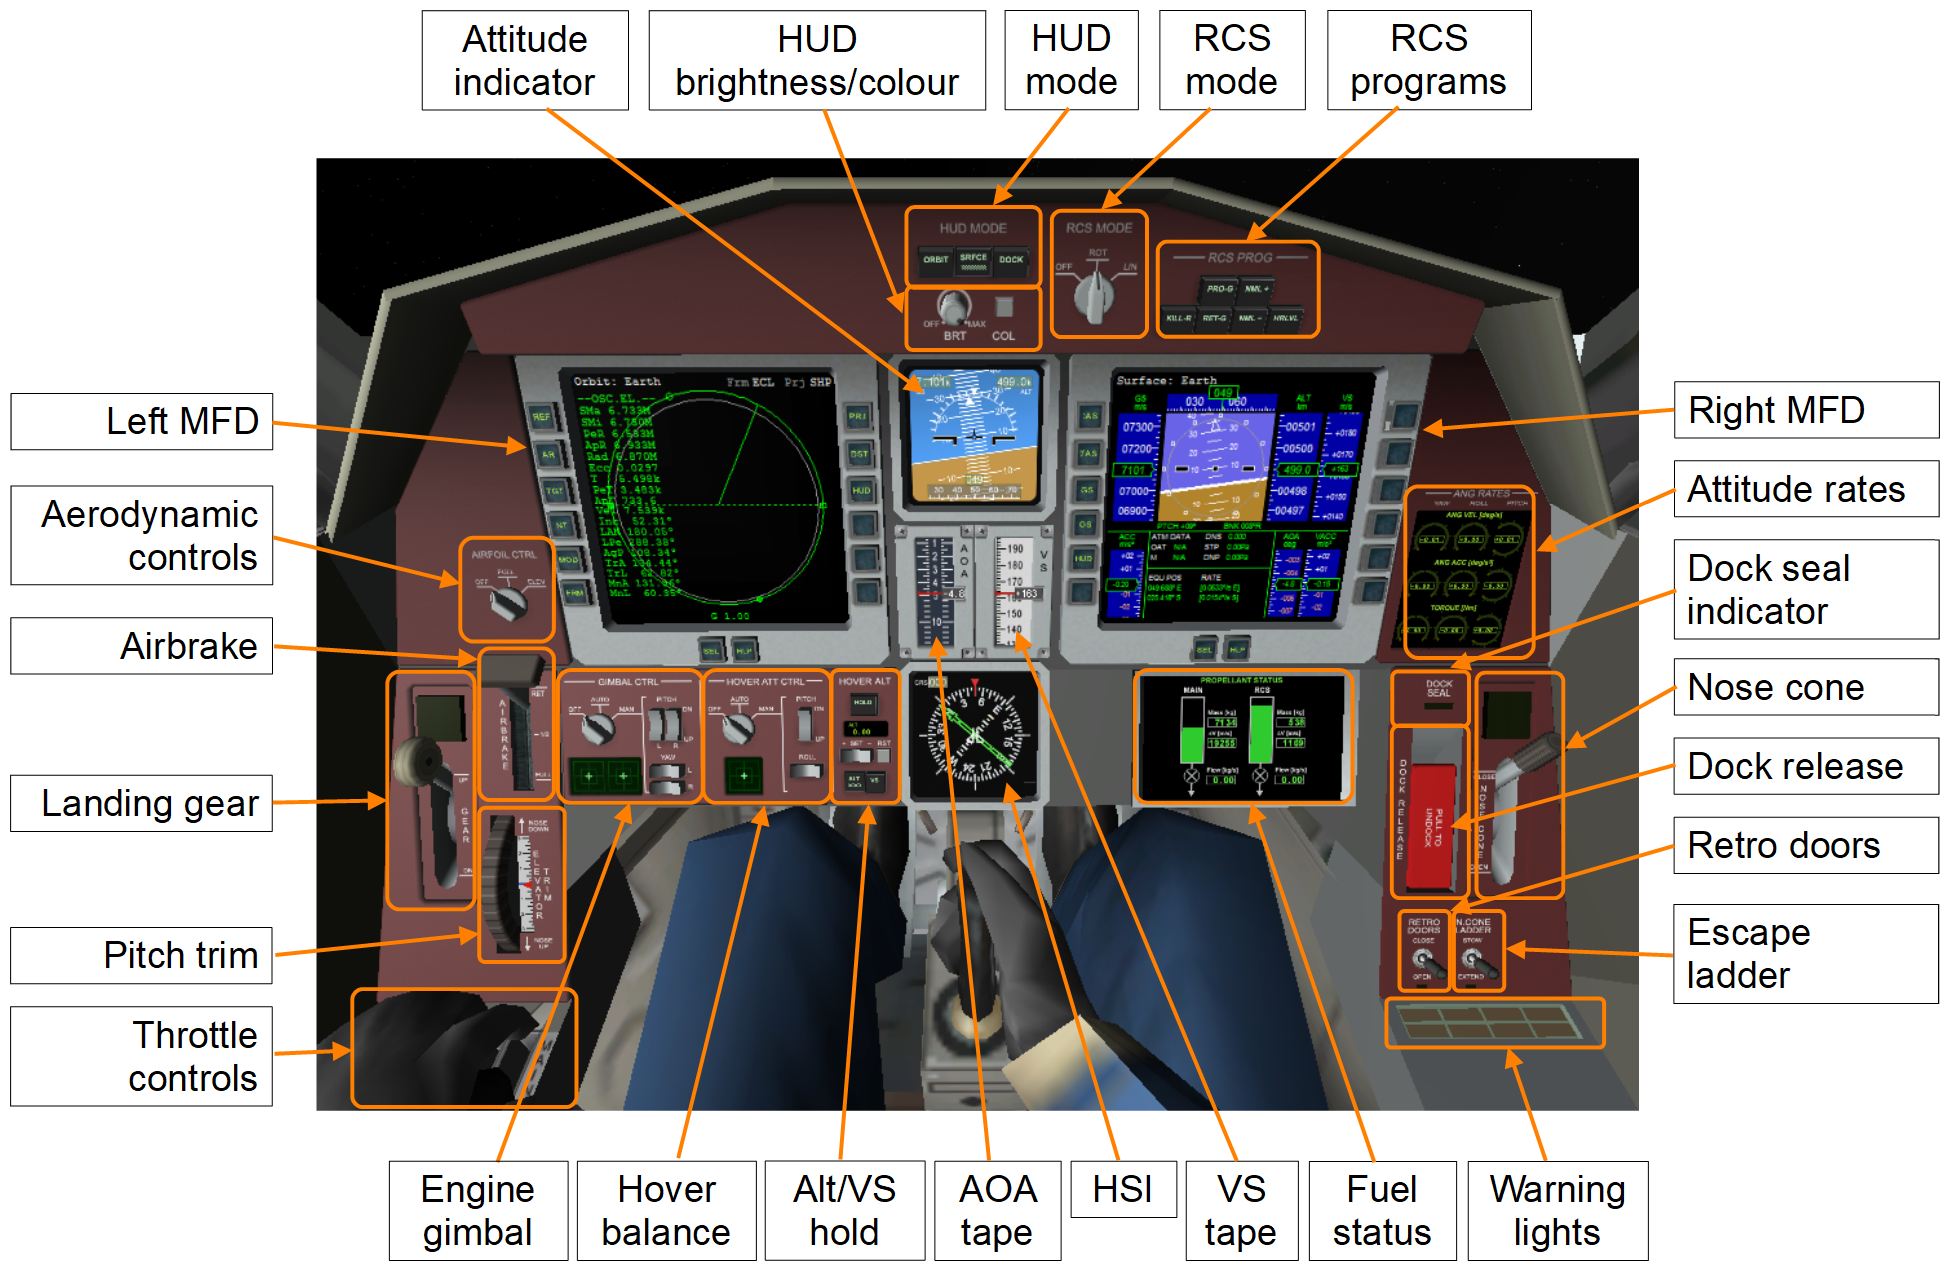
\includegraphics[width=\hsize]{dg_VC0.png}
  \caption{Delta-glider virtual cockpit: overhead and main panels.}
\end{figure}

\noindent
\textbf{Moving between VC positions}\\
The default virtual cockpit position places you in the pilot's seat, behind the pane of the head-up display and with access to all instruments and flight controls. You can however also switch your position to any of the 4 passenger seats in the cabin, for example to experience the replay of a recorded flight from a passenger's perspective.

\begin{figure}[H]
  \centering
  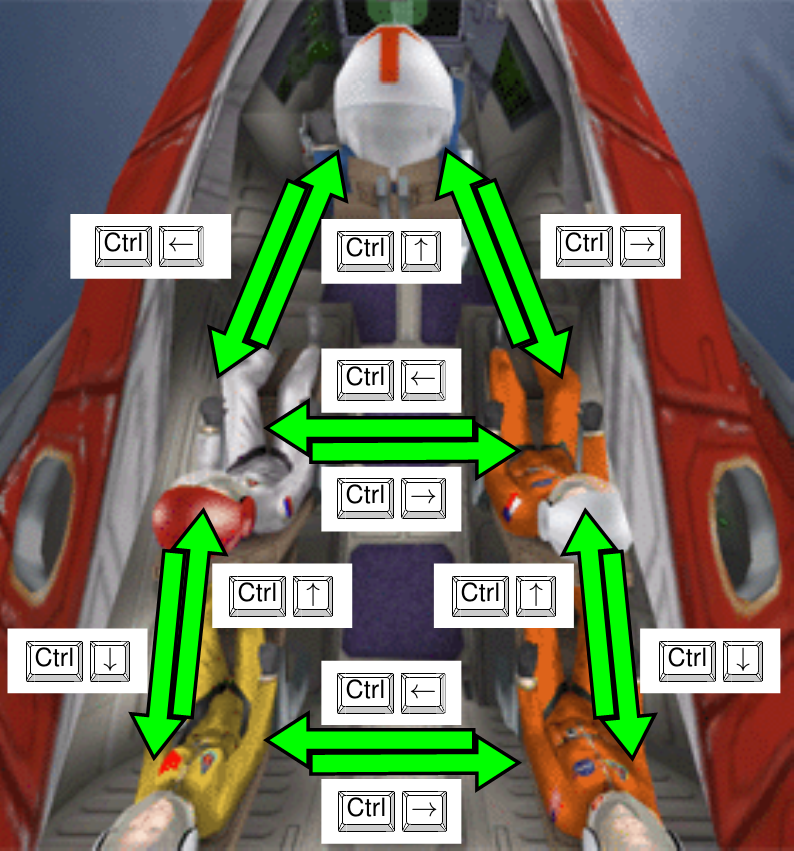
\includegraphics[width=0.5\hsize]{dg_vc_pos.png}
  \caption{Transition paths between VC positions.}
\end{figure}

\noindent
To switch to a different VC position, use \Ctrl\UArrow\DArrow\LArrow\RArrow key combinations. The picture illustrates the different jump paths.


\subsubsection{Propulsion}
\paragraph{Main engines}
The Delta-glider's main propulsion is provided by two rear-mounted engines generating a maximum thrust of 160 kN each in vacuum. At maximum thrust, the main engines accelerate a fully loaded vessel at 12.9 m/s$^{2}$. The trust level can be adjusted continuously between zero and maximum (keyboard shortcuts \Ctrl\keystroke{+}$_{Num}$ and \Ctrl\keystroke{-}$_{Num}$) or with the throttle sliders in the 2-D panel or virtual cockpit. The sliders also allow to set the thrust levels individually for both engines. Differential engine thrust will however result in a yaw moment unless compensated for with the appropriate gimbal setting (see below).\\
The main engines are fuelled from the Delta-glider's main fuel tank, with a capacity of 12900 kg (propellant + oxidiser) for the DG and 10400 kg for the DG-S. At a vacuum specific impulse of Isp = 4 x 10$^{4}$ m/s this leads to a maximum burn time of 1612 s (DG) and 1300 s (DG-S), and a maximum delta-v budget of $\Delta$v = 2.93 x 10$^{4}$ m/s (DG) and $\Delta$v = 1.96 x 10$^{4}$ m/s (DG-S). The DG-S value rises to $\Delta$v = 2.23 x 10$^{4}$ m/s for an empty scramjet propellant tank. Note however that the DG and DG-S main tank also feeds the retro and hover engines, affecting the maximum $\Delta$v attainable from the main engines in practice.\\
\\
\textbf{Main engine gimbal control}\\
Each main engine is mounted on a gimbal platform with a rotation range of $\pm$5.0° in pitch and $\pm$7.4° in yaw, providing thrust vector capability. Engine gimbal configuration can be used to provide angular momentum in pitch, yaw and roll during main engine burns. The torque generated by thrust vectoring at maximum deflection and maximum main engine thrust is 215 kNm (pitch), 317 kNm (yaw) and 27.9 kNm (roll) - all values for a fully loaded DG. The roll torque is relatively small because the main engines are mounted close to the vessel centreline.

\begin{figure}[H]
  \centering
  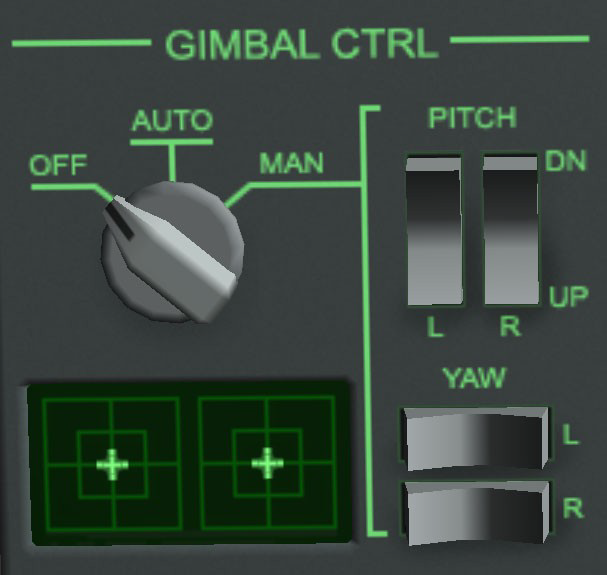
\includegraphics[width=0.4\hsize]{dg_main.png}
  \caption{Main engine gimbal controls and gimbal position indicators.}
\end{figure}

\noindent
Engine gimbal in the yaw axis can provide compensation for the torque induced by thrust differentials in the two main engines. The yaw gimbal range is designed so as to compensate for torque generated by a single main engine burn in case of one of the engines failing. However, remember that while cancelling the induced torque, yaw gimbaling will add lateral linear momentum, resulting in a non-zero slip angle.\\
The gimbal controls are located at the lower left main panel (GIMBAL CTRL). The mode selector dial has three settings: OFF - engines are centered; AUTO - gimbal settings are commanded from pilot control input, and yaw gimbal automatically compensates for main engine thrust differential; MAN - gimbal settings are adjusted manually.\\
In MAN mode, the gimbal settings for pitch and yaw can be set manually with the rocker switches right of the selector dial. The left and right engines can be gimbaled individually. To tilt both engines simultaneously, click between a switch pair.\\
In AUTO mode, the gimbal settings follow the pilot's pitch, yaw and roll commands from joystick or keyboard controls. They provide automatic thrust vectoring for additional angular acceleration during main engine burns. Thrust vectoring can be used in conjunction with aerodynamic control surfaces or RCS attitude control, or on its own.\\
The display below the selector dial shows the commanded (outer cross-hair) and current pitch and yaw gimbal positions (inner cross-hair) for both engines. The outer box represents maximum gimbal deflection, the inner box half that value. Note that the gimbal mounts rotate at a rate of 3.4°/s, so there can be a delay until the commanded deflection is achieved.

\paragraph{Retro engines}
The DG is equipped with a pair of small forward-facing engines installed in the leading wing edges for providing reverse thrust. The retro engines are protected by covers during high airspeed atmospheric flight. Once free of the atmosphere or at low airspeed (e.g. during a vertical landing approach), the covers must be opened before activating the thrusters. The covers are opened and closed with the "Retro doors" switch in the lower right panel of the VC and 2-D cockpit view. Do not forget to close the covers before reentry! The retro engines are useful to decelerate the DG without the need to turn the vessel to engage its main engines, e.g. to cancel forward motion when aligning the position above a landing pad.

\begin{figure}[H]
  \centering
  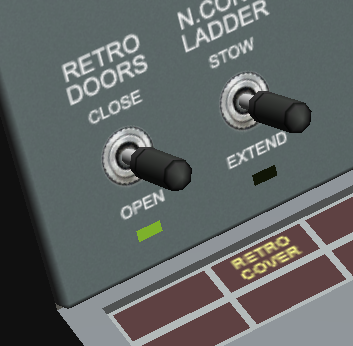
\includegraphics[width=0.4\hsize]{dg_retro.png}
  \caption{Retro cover activation switch and retro warning light in the VC.}
\end{figure}

\noindent
The retro engines are activated by moving the main engine throttles below the zero position into the red "RET" area. Keyboard shortcut: \Ctrl\keystroke{-}$_{Num}$. If the main engines are active, they must be cut before the retro engines can be activated. To cut either active main or retro engines and return the throttles to the zero position, press \keystroke{*}$_{Num}$.\\
Each retro engine produces a vacuum thrust of 34 kN. At maximum thrust, the retro engines accelerate a fully loaded DG by 2.7 m/s$^{2}$ in backward direction. Note that you can also use the RCS (see below) in translational mode for providing backward thrust, but the retro engines produce significantly higher thrust.

\paragraph{Hover engines}
Three downward-facing engines are mounted in the lower part of the fuselage, providing limited vertical take-off and landing capability. The forward positioned engine generates a thrust of 110 kN, and each of the two rear engines generates 36.3 kN, leading to an upward thrust balanced at the centre of gravity. For a fully loaded DG, the resulting acceleration at full thrust is 7.35 m/s$^{2}$ in vacuum (less in an atmosphere), too little to overcome Earth surface gravitational acceleration, but sufficient on the Moon and Mars. To lift off on hover engines from Earth at sea level, the total vessel mass must be lower than 14880 kg by reducing the amount of fuel carried.\\
\\
\textbf{Hover attitude control}\\
The relative thrust generated by the three hover engines can be modulated within small margins to produce a force differential that induces a pitch or bank moment and can be used to change the vessel attitude during hover operation. The controls for hover attitude modulation are located in the lower left panel (HOVER ATT CTRL) to the right of the main engine gimbal controls.

\begin{figure}[H]
  \centering
  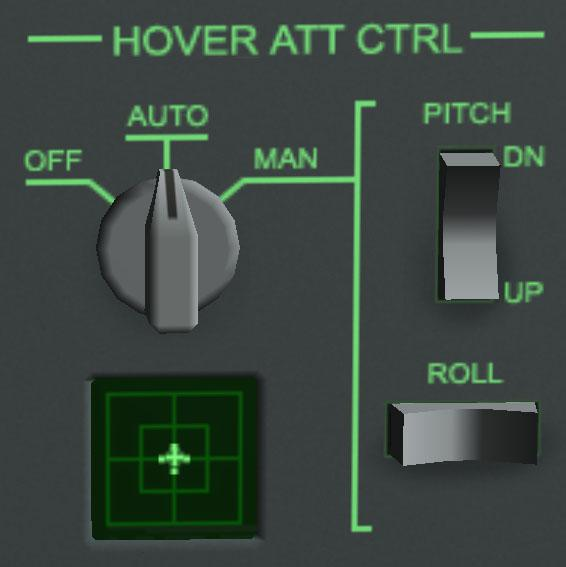
\includegraphics[width=0.4\hsize]{dg_hover.jpg}
  \caption{Hover attitude modulation controls.}
\end{figure}

\noindent
The selector dial has three positions: OFF - attitude control disabled, all thrusters engage at balanced level; AUTO - automatic attitude balancing mode commanded by user input; MAN - manual pitch and bank modulation.\\
In AUTO mode, the target attitude is commanded by the manual input controls (keyboard or joystick). With controls in neutral position, the differential hover thrust is set to keep the vessel level with the local horizon. Engaging pitch and bank controls commands a target pitch or bank attitude, maintained by differential hover thrust. This change in attitude creates a horizontal component of thrust from the hover engines, resulting in a horizontal acceleration. Centering the stick again zeros the horizontal acceleration, maintaining the current horizontal velocity (in the absence of an atmosphere). This mode is useful for adjusting the vessel position over a target touchdown point during VTOL operations.\\
The automatic hover attitude mode should generally be used in conjunction with the hover hold altitude/vertical speed mode, because the vertical component of hover thrust is affected by vessel attitude, resulting in a change in vertical speed. The hover hold altitude/vertical speed mode automatically adjusts for this.\\
Note that the automatic hover attitude mode is only operational for vessel pitch and bank angles < 30°. At higher angles, the automatic mode disengages.\\
The hover attitude control system modulates the differential thrust of the hover engines so that the total thrust from the three engines is maintained. This means that a thrust reserve beyond the commanded mean hover level is required to service the modulation requests. If the mean hover level is set too close to full or zero thrust to provide the required reserves, attitude control is disabled.\\
RCS rotational attitude control programs should be disengaged before activating hover attitude control to avoid conflicts between the two attitude control loops.\\
In MAN mode, the commanded pitch and roll angles are set directly with the two rocker switches to the right of the selector dial.\\
The display below the dial shows the current and commanded hover pitch and bank attitudes. The inner and outer box shown in the display indicate an attitude angle of 5° and 10°, respectively.\\
\\
\textbf{Hover hold altitude/vertical speed control}\\
The hover hold altitude/vspeed program allows to automatically adjust hover engine thrust for maintaining a specified altitude or vertical speed. The controls for activating the program and setting the parameters (HOVER ALT) is located in the lower left panel, right of the hover attitude controls.

\begin{figure}[H]
  \centering
  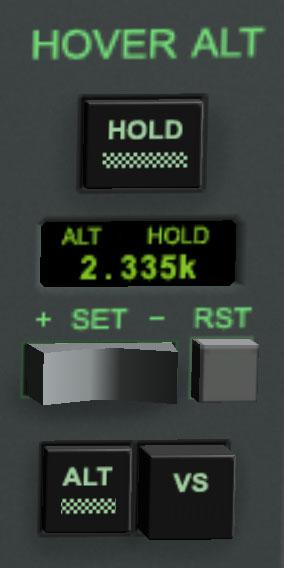
\includegraphics[width=0.2\hsize]{dg_hover_alt.jpg}
  \caption{Hover hold altitude/vspeed panel.}
\end{figure}

\noindent
Switch between altitude or vertical speed modes with the ALT/VS buttons at the bottom of the panel. The display shows the current target setting of the selected parameter in meters above ground (ALT) or in m/s (VSPD). The value can be adjusted with the SET +/- rocker switch. In ALT mode, the RST button sets the target altitude to the current vessel altitude. In VSPD mode, the RST button sets the target vertical velocity to 0.\\
Press the HOLD button to activate the selected hover program. Pressing the button again disengages the program. The vessel will maintain the hover thrust setting at that point.\\
When switching directly from an active ALT mode to VS mode, the target vertical speed is set to the current vertical speed. Likewise, switching from active VS to ALT mode sets the target to the current altitude.\\
The hold altitude/vertical speed mode requires the vessel to be approximately level with the local horizon. It is advisable to use it in combination with the automatic hover balance mode. At significant pitch or bank angles the available hover thrust may not be sufficient to maintain the commanded value.\\
The hover hold altitude/vertical speed mode is most useful in surface proximity of a planetary body without an atmosphere, where vertical take-off and landing is required. The vertical speed mode can be used for controlled launches and soft touchdowns.

\paragraph{Scramjet engines (DG-S only)}
The DG-S version of the Delta-glider is equipped with a pair of air-breathing scram engines mounted underneath the fuselage, in addition to its rocket engines. They can provide efficient propulsion in Earth's atmosphere in a limited pressure and airspeed regime.\\
Scramjets are a variant of ramjet engines. A ramjet has no moving parts - unlike standard turbojet engines, the compression of the incoming air prior to combustion is achieved purely from the vessel's airspeed. In ramjets, the air is decelerated to subsonic speeds before combustion, while in scramjets combustion occurs at supersonic speeds.\\
This design means that scramjets (and to a lesser degree, ramjets) can only operate at high airspeeds. They can't be used to take off from the ground, so additional propulsion is required at low speeds until the scramjets can take over. For the DG-S, the operational speed for the scramjet engines is approximately Mach 3-8. At the lower limit the scramjets lose efficiency due to low air compression. At the upper airspeed limit, the limiting factor is the engine temperature, which must be kept within material constraints by reducing the ingoing airflow.\\
At optimal conditions, each scramjet engine generates approximately 325 kN of thrust, roughly twice the power of the rocket main engines. The scramjets are significantly more fuel-efficient than the main engines, because they don't require oxidizer to be carried along. This is reflected in a value of specific impulse of approximately Isp = 1 x 10$^{5}$ m/s at optimal operational parameters. The maximum fuel mass flow rate per engine supported by the fuel pumps is 3.0 kg/s.

\paragraph{Reaction control system}
The Reaction Control System (RCS) consists of set of 16 small thrusters arranged to provide attitude and linear control during orbital operations. RCS thrusters are engaged in pairs, either in rotational mode to induce an angular moment around one of the vessel principal axes, or in translational mode to provide a linear moment in the direction of one of the axes. Each thruster generates 3.5 kN of thrust. In linear mode, this results in an acceleration of 0.25 m/s$^{2}$ from a thruster pair for a fully loaded DG. In rotational mode, the generated torque ranges from 30 kNm (yaw and roll) to 40 kNm (pitch), resulting in an angular acceleration of 3°/s$^{2}$ (yaw), 9°/s$^{2}$ (roll) and 6°/s$^{2}$ (pitch) for a fully loaded DG.

\begin{figure}[H]
  \centering
  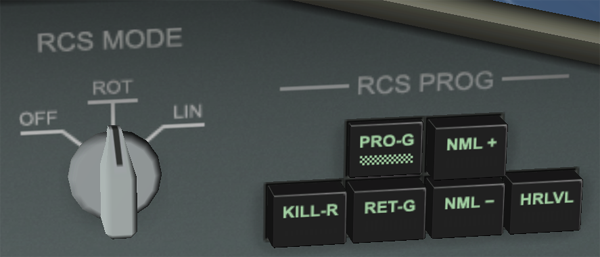
\includegraphics[width=0.6\hsize]{dg_rcs.png}
  \caption{RCS mode selector dial and attitude program switches in the VC.}
\end{figure}

\noindent
%TODO add section link
The RCS mode is switched between rotational and linear modes with the RCS MODE selector dial (keyboard shortcut \keystroke{/}$_{Num}$). The keyboard and joystick commands for engaging RCS along specific axes can be found in TODO. RCS thrusters are engaged either at full power, or at 10\% of full power for fine adjustments, using keyboard commands in combination with \Ctrl.\\
%TODO add section link
The DG supports the full range of default RCS attitude programs (prograde/retrograde, normal/antinormal to the orbital plane, level with respect to local horizon, and kill rotation). See TODO for an overview of the attitude programs and how to engage them.

\paragraph{Propellant management}
The propellant management display is located on the lower left of the front panel (PROPELLANT STATUS). It shows the fill level fuel mass of the installed propellant tanks (main, RCS, and scram for the DG-S). It also shows the $\Delta$v equivalent of the remaining fuel resources, and the current mass flow rate from each tank.

\begin{figure}[H]
  \centering
  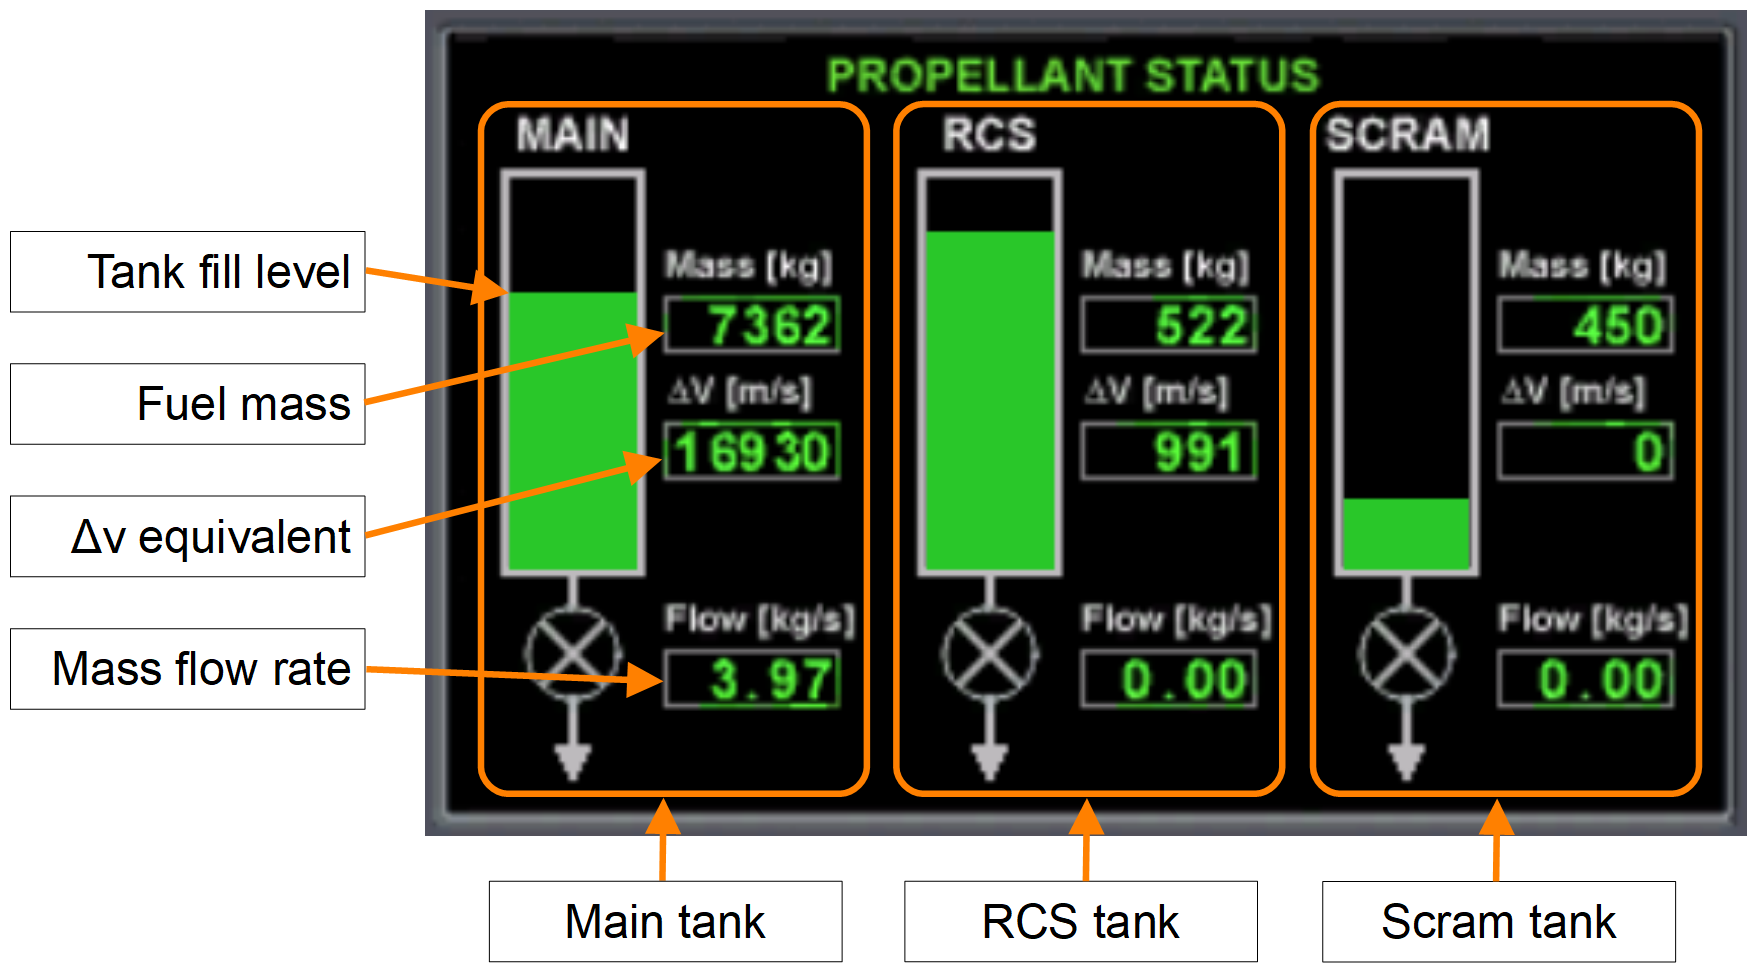
\includegraphics[width=\hsize]{dg_prop_mgmt.png}
  \caption{DG-S propellant management display.}
\end{figure}

\subsubsection{Avionics}
%TODO add section link
Avionics displays and controls are located on the DG main panel. The primary avionics interfaces are the two multifunctional displays (MFDs). For a description of the available MFD modes and operation see TODO. In addition to the MFDs, the DG provides some secondary avionics instruments.

\paragraph{Head-up display}
%TODO add section link
The DG's head-up display (HUD) consists of a glass pane in the pilot's forward line of sight, suspended from the overhead panel, and a projector located above the pilot position. The HUD supports Orbiter's standard display modes (\textit{Surface}, \textit{Orbit} and \textit{Docking} - see TODO). The mode can be selected with the three HUD MODE buttons in the centre of the front panel (keyboard shortcut: h). When not required, the HUD can be retracted with the HUD RET/EXT switch in the overhead panel (keyboard shortcut: \Ctrl\keystroke{H}). This also turns off the projector.

\begin{figure}[H]
  \centering
  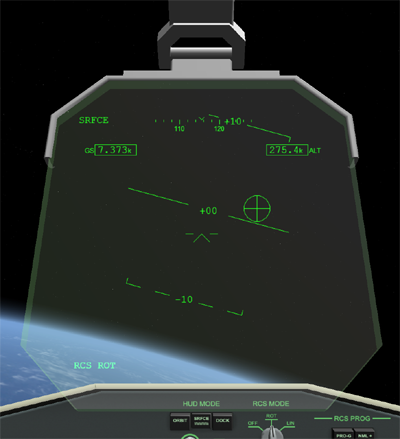
\includegraphics[width=0.4\hsize]{dg_hudpane.png}
  \caption{DG HUD pane in the VC.}
\end{figure}

\noindent
Below the HUD mode selector buttons is a dial for adjusting the projector brightness and a toggle to cycle through the available display colours (keyboard shortcut: \Alt\keystroke{H}). Switching colours may improve visibility under different viewing conditions.

\begin{figure}[H]
  \centering
  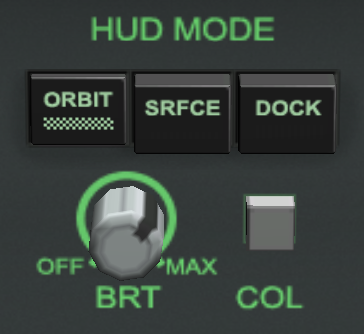
\includegraphics[width=0.25\hsize]{dg_hudmode.png}
  \caption{HUD mode selector and brightness/colour controls on the front panel.}
\end{figure}

%TODO img side-by-side?

\begin{figure}[H]
  \centering
  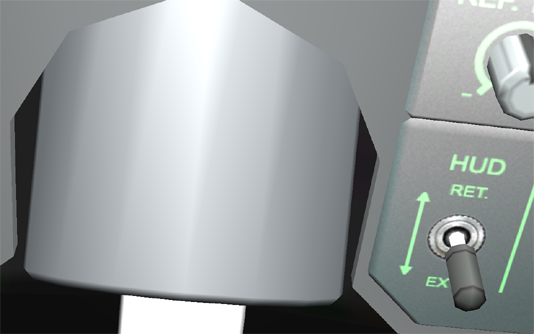
\includegraphics[width=0.4\hsize]{dg_hudctrl.png}
  \caption{HUD projector and HUD extend/retract control on the overhead panel.}
\end{figure}


\paragraph{Attitude indicator}
The \textit{attitude indicator} is located in the top centre of the main panel. It shows pitch and roll attitude relative to the local horizon, as well as heading, altitude and airspeed readouts. The attitude indicator replicates the attitude display of the \textit{Surface} MFD mode. This potentially frees up an MFD instrument for displaying a different mode.

\begin{figure}[H]
  \centering
  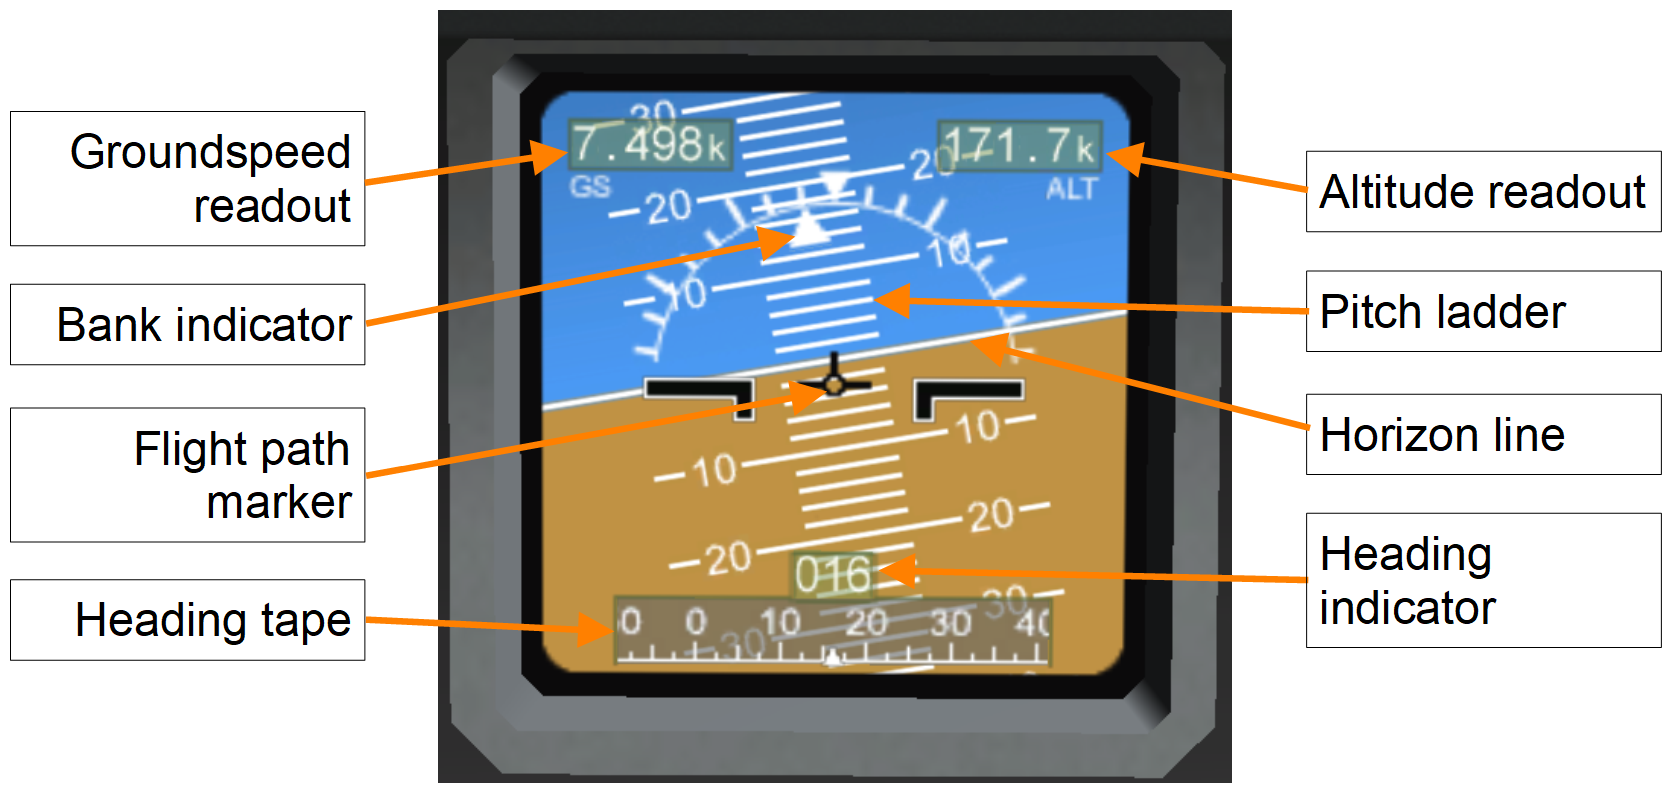
\includegraphics[width=0.8\hsize]{dg_att_ind.png}
\end{figure}

\paragraph{Horizontal situation indicator}
The \textit{horizontal situation indicator} (HSI) is located in the bottom centre of the main panel. It shows a compass rose with the current heading indicated with a marker at the 12 o'clock position. The HSI receives input from the NAV1 nav-radio receiver and can display course information from VOR transmitters or approach data from ILS transmitters.

\begin{figure}[H]
  \centering
  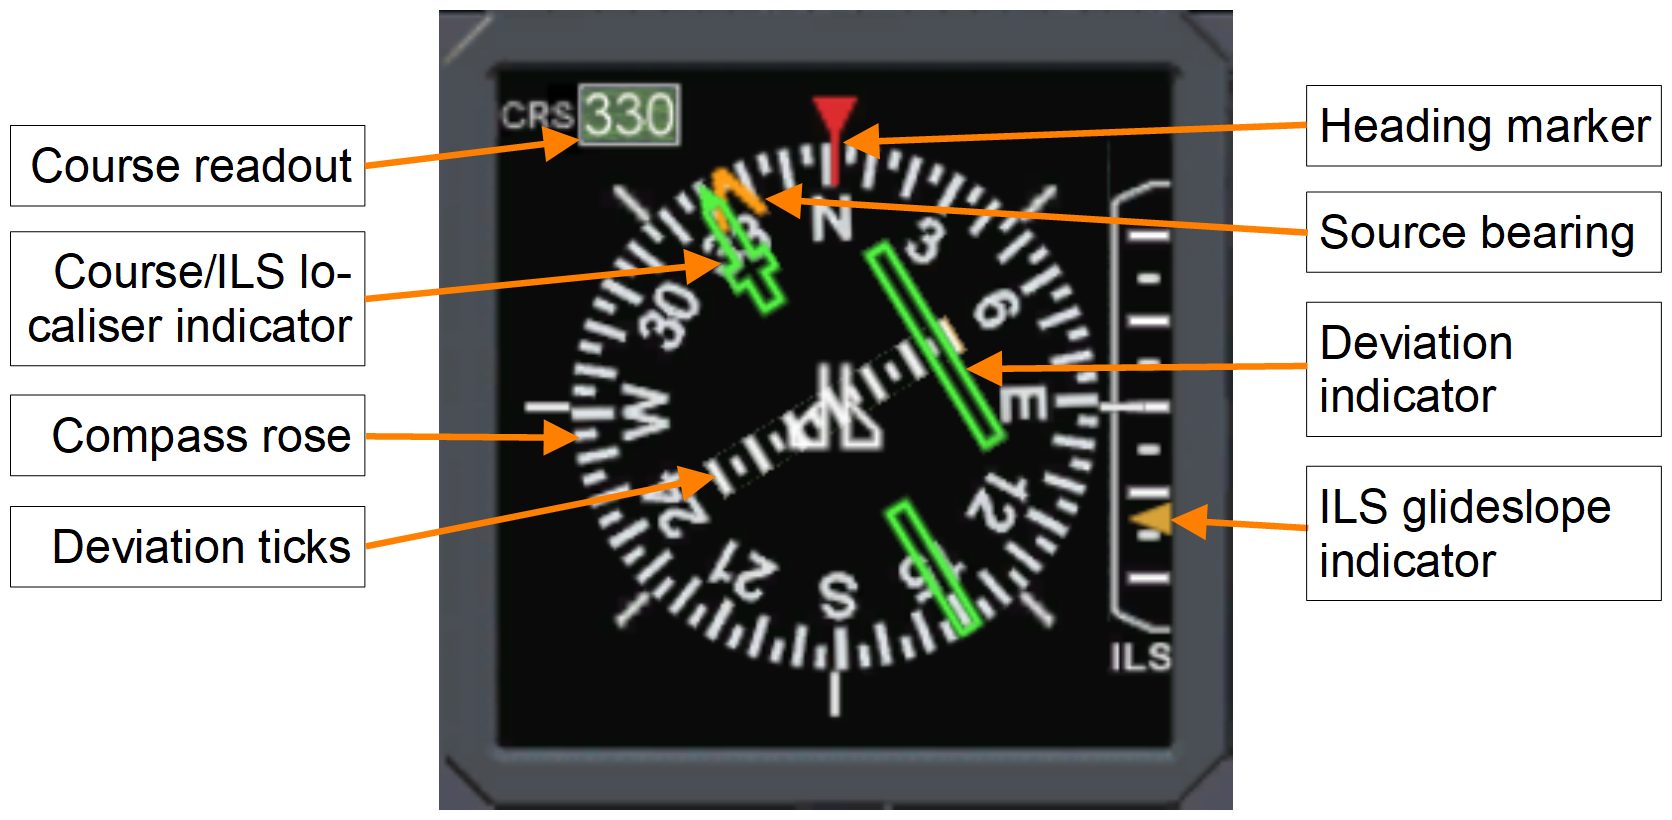
\includegraphics[width=0.8\hsize]{dg_hsi.png}
\end{figure}

\noindent
When a transmitter signal is received, the orange \textit{source bearing} bug indicates the bearing to the transmitter source.\\
%TODO add section link
The green \textit{course} and \textit{deviation} indicator needle can be used to display a target heading or the ship's position relative to a VOR radial. It is used in conjunction with the DG's atmospheric autopilot (AAP) - see TODO\\
When the AAP \textit{heading} mode is activated, the course indicator represents the target heading. It can be rotated with the rocker switch in the AAP controls below to the HDG/CRS readout. The autopilot will try to keep the vessel's heading aligned with this target heading, i.e. will keep the course needle pointing to 12 o'clock. This mode is independent of a VOR transmitter and also works if no VOR signal is received.\\
When the AAP heading mode is disengaged, the course indicator can still be rotated with the AAP rocker switch, but it will not activate a heading response. If a VOR signal is received, the indicator represents a radial to or from the VOR signal source, and the deviation indicator shows the ship's position relative to the radial. As the ship approaches the radial, the deviation indicator moves towards the centre of the display. If the AAP heading mode is activated on intercept, the vessel will turn into the selected radial and keep the deviation indicator centered.\\
If NAV1 is tuned to an ILS transmitter, the course indicator is fixed to the runway approach path direction and cannot be rotated with the AAP heading target. The deviation marker shows the direction of the localiser plane (the vertical plane aligned with the runway centreline) relative to the ship's position. In addition, the glideslope indicator becomes active and shows the glideslope plane relative to the ship's vertical position. The glideslope needle below the centre position indicates too high an approach, the needle above centre position indicates a low approach.


\paragraph{Angle of attack and vertical speed indicator}

\begin{figure}[H]
  \centering
  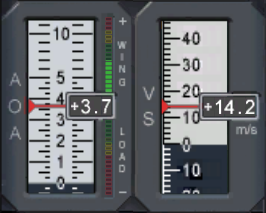
\includegraphics[width=0.3\hsize]{dg_tapes.png}
  \caption{AOA tape with wing load indicator and vertical speed tape.}
\end{figure}

\noindent
\textbf{AOA tape}\\
Below the attitude indicator are the angle of attack (AOA) and vertical speed (VS) tapes. AOA is the vertical component of the angle between the ship's centre line (forward direction, +z axis in the local vessel frame) and its flight path through the atmosphere (relative wind). It represents the angle at which the DG's wing hits the oncoming air and is an important indicator for estimating lift and drag. Higher AOA values generate higher lift and drag forces up to a limit (critical AOA), after which the airflow starts to separate from the upper wing surface, rapidly decreasing the generated lift. The AOA tape has a range of $\pm$40° (with higher resolution within $\pm$5°) but the digital readout works beyond that limit.\\
\\
\textbf{Wing load indicator}\\
The AOA tape also includes a wing load indicator (currently only available in the 2-D panel version). Wing load in this context is to be understood as lift force divided by wing area. Wing load can reach high values during high-AOA manoeuvres at high airspeeds. Exceeding the DG's structural limits can lead to airframe damage. The wing load indicator consists of a line of coloured LEDs, where green = within limits, yellow = approaching limit, red = exceeding limits. Note that the magnitude of the negative wing load limit (at negative AOA) is lower than that of positive wing load.\\
\\
\textbf{Vertical speed tape}\\
Located next to the AOA tape is the vertical speed tape and readout. Vertical speed is displayed in m/s up to a range of $\pm$10$^{4}$ m/s. Beyond that, the readout shows vertical speed in km/s, while the tape displays the fractional m/s remainder. Vertical speed is measured relative to the surface; it does not depend on an atmosphere.\\
Both AOA and vertical speed readouts are also available in the MFD \textit{Surface} mode.


\paragraph{Atmospheric autopilot}
The atmospheric autopilot (AAP) engages main thrusters and aerodynamic control surfaces to maintain commanded airspeed, altitude and/or heading in an atmosphere. The AAP control interface is located in the top left of the main panel. The digital readouts show the commanded values for altitude, speed and heading. They can be adjusted with the rocker switches below each display. The toggle switches left of the readouts activate and deactivate the corresponding autopilot component.

\begin{figure}[H]
  \centering
  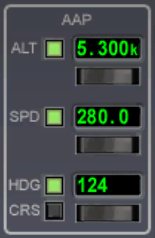
\includegraphics[width=0.25\hsize]{dg_aap.png}
  \caption{AAP interface.}
\end{figure}

\noindent
Note that not all commanded settings result in a stable flight condition. For example, if the commanded airspeed is too low, the generated lift may not be sufficient to maintain the commanded altitude.\\
%TODO add section link
An alternative way to access the AAP is via the script interface on the \textit{Console} MFD mode (see TODO). Note however that the console invokes a separate instance of the AAP, so both methods should not be used simultaneously to avoid conflicts.

\subsubsection{Thermal management}
During orbital operations the DG can unfold a pair of radiator panels to emit excess heat. A coolant loop collects thermal energy from the cabin and onboard electrical systems and transports it to the radiators. When the radiators are stowed, a limited amount of heat can also be deposited in the propellant stores. A display in the overhead panel shows the operation of the coolant system, including the temperatures at different positions in the loop. Controls consist of a switch to turn the coolant pump on and off, a dial to set the pump rate, and a dial to set the target reference temperature. To maintain the target temperature, the control system adjusts the radiator/bypass ratio of the coolant flow. The radiator is extended/retracted with a switch below the thermal control display. The efficiency of the radiators is reduced if they are irradiated directly by sunlight. Likewise, heat absorption by the DG's fuselage from solar irradiation depends on the irradiated cross section. This should be taken into account when setting the ship's attitude relative to the sun during orbital operations.

\begin{figure}[H]
  \centering
  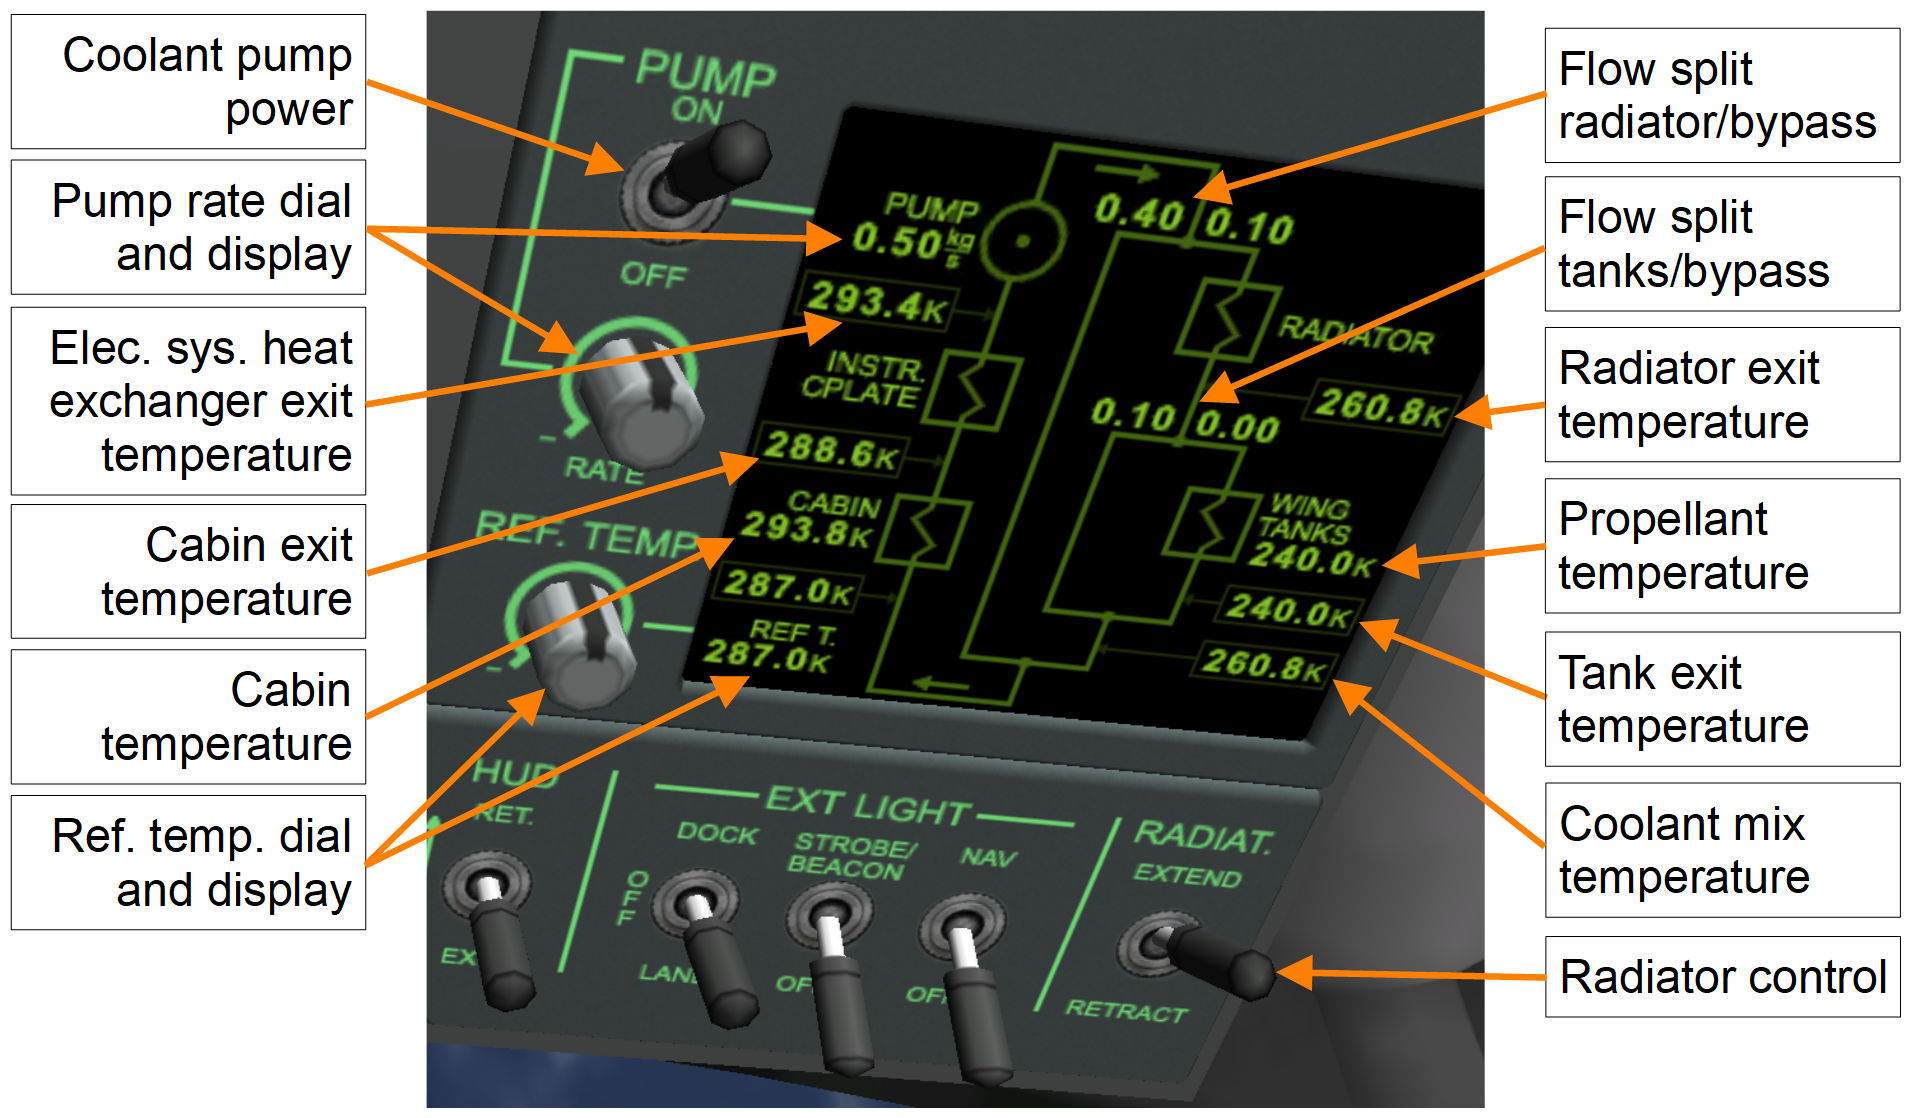
\includegraphics[width=\hsize]{dg_temp_mgmt.png}
\end{figure}

\subsubsection{Life support system}
The life support system regulates atmospheric pressure in the cabin and the airlock from two nitrogen/oxygen (N$_{2}$/O$_{2}$) tanks. Two valves open and close the air supply from the tanks. In addition, there are three pressure relief valves (V1, V2, V3) which equalise pressure between cabin and airlock (V2), between cabin and environment (V1), and between airlock and environment (V3). V2 should be open before opening the inner airlock. V1 should be open before opening the cabin hatch, and V3 should be open before opening the outer airlock. The N$_{2}$/O$_{2}$ tanks should be cut off before opening the hatch or the airlock doors.\\
Pressure readouts for cabin, airlock and environment are provided on the left of the overhead panel. The panel also provides controls for the N2/O2 tanks and the relief valves. The cabin hatch and inner/outer airlock doors are controlled from this panel as well.

\begin{figure}[H]
  \centering
  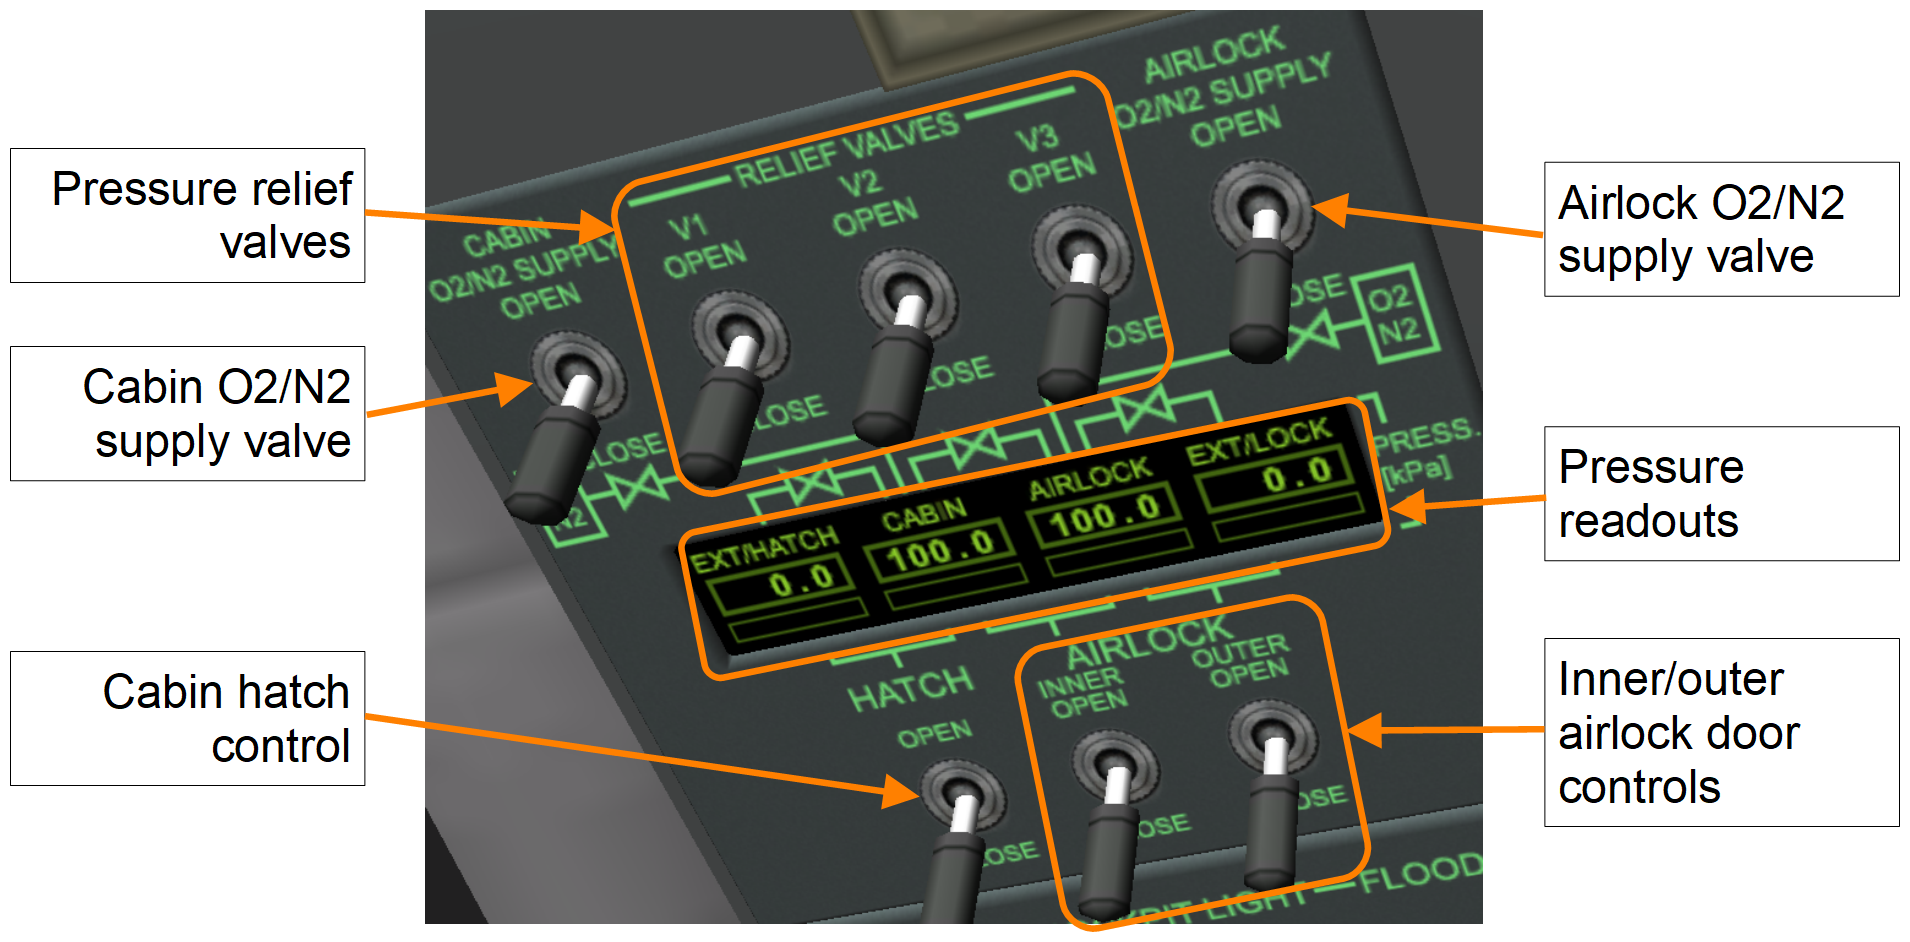
\includegraphics[width=\hsize]{dg_life_supp.png}
\end{figure}

\subsubsection{Cockpit and external lighting}
The lighting controls are located in the overhead panels. On the left are the instrument light controls (on/off, brightness) and floodlight controls (white/red). On the right are the external light and navigation beacon controls.

\begin{figure}[H]
  \centering
  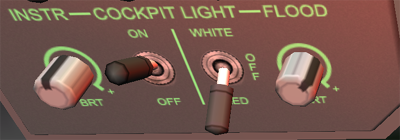
\includegraphics[width=0.5\hsize]{dg_light_int.png}
  \caption{Instrument light on/off and brightness, cockpit floodlight on/off and brightness (left overhead panel).}
\end{figure}

\noindent
A spotlight mounted beneath the nosecone can be configured as a landing light ("LAND" - angled downward) or docking light ("DOCK" - pointing forward). The DG also has a set of navigation lights (green - starboard, red - port, white - stern) and strobes.

\begin{figure}[H]
  \centering
  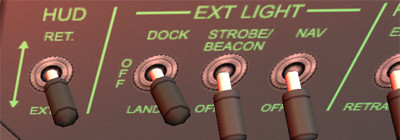
\includegraphics[width=0.5\hsize]{dg_light_ext.png}
  \caption{Docking/landing lights, strobes and navigation lights (right overhead panel).}
\end{figure}

\noindent
Note that for the cockpit floodlights and eternal landing/docking lights to work, \textit{local light source} support must be enabled on the \textit{Visual effects} tab of the Orbiter Launchpad dialog.

\begin{figure}[H]
  \centering
  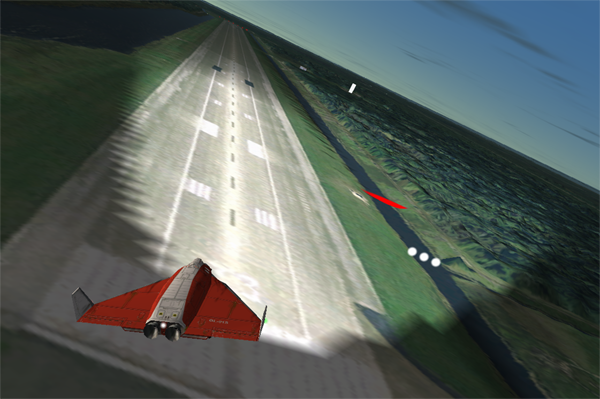
\includegraphics[width=\hsize]{dg_light_land.png}
  \caption{DG with landing lights.}
\end{figure}


\subsubsection{Script interface}
%TODO html doc link?
The DG has access to the standard functions provided by the Orbiter-Lua script interface (see .\textbackslash Html\textbackslash orbiter.chm, chapter \textit{Orbiter Scripting} for an overview of the script interface and .\textbackslash Orbitersdk\textbackslash doc\textbackslash orbiter\_lua.chm for details of the API). The vessel-related functions can be used to query flight parameters and to control spacecraft operations.\\
The script interface can be accessed in two ways:

\begin{itemize}
%TODO check keys are correct
\item via the \textit{Terminal} MFD mode. Make sure that the \textit{LuaMFD} plugin module is activated in the \textit{Modules} tab of the Orbiter Launchpad. This will add the Terminal mode to the list of available MFD modes (open with keyboard shortcut: \Shift\keystroke{F4} + \Shift\keystroke{T}). Script commands can be entered with the INP button (keyboard shortcut: \Shift\keystroke{I}). For vessel-based methods, the terminal provides object "V" to represent the active vessel (equivalent to command V = vessel.get\_focusinterface() ). You can use this object to access the DG, for example

\begin{lstlisting}[language=OSFS]
term.out(V:get_mass())
\end{lstlisting}

\item via the Console window. Make sure that the LuaConsole plugin module is activated in the Modules tab of the Orbiter Launchpad. During a simulation session, open the console with Lua console window from the Custom functions list (\Ctrl\keystroke{F4}). To access your DG, you first have to create an interface object, and then use it to access vessel functionality, e.g.

\begin{lstlisting}[language=OSFS]
dg = vessel.get_focusinterface()
term.out(dg:get_mass())
\end{lstlisting}

\noindent
Of course you can create an interface to any other vessel in the simulation as well, using

\begin{lstlisting}[language=OSFS]
v = vessel.get_interface(<name>)
\end{lstlisting}

\end{itemize}

\paragraph{Atmospheric autopilot (script version)}
%TODO add section link
The DG provides a vessel-specific script API extension that implements the atmospheric autopilot discussed in TODO). This script extension is loaded automatically when opening a Terminal MFD in the DG, but must be loaded explicitly in the Console window and connected with the correct vessel:

\begin{lstlisting}[language=OSFS]
run('dg/aap')
setvessel(vessel.get_focusinterface())
\end{lstlisting}

\noindent
There is nothing to stop you from trying to invoke the AAP for a different vessel type, but the parameters are tuned to the DG mass, inertia and aerodynamic properties, so it is unlikely to work well on a different spacecraft without modification.\\
The code for the autopilot functions is located in file .\textbackslash Script\textbackslash DG\textbackslash aap.lua. Feel free to edit the code to modify the behaviour of the autopilot. The script interface makes it easy to change things and test them directly in Orbiter.\\
Note that the script interface creates a new instance of the autopilot that is independent of the version accessed via the DG instrument panel. Avoid having both active simultaneously to avoid conflicts.\\
\\
\textbf{Altitude module}\\
The altitude sub-module of the AAP is engaged with

\begin{lstlisting}[language=OSFS]
aap.alt(<tgtalt>)
\end{lstlisting}

\noindent
where \textit{<tgtalt>} is the target altitude [m] the autopilot is commanded to reach and maintain. The target altitude can be modified either by calling the aap.alt function again with a different value, or by overwriting the aap.tgtalt parameter:

\begin{lstlisting}[language=OSFS]
aap.tgtalt = <newalt>
\end{lstlisting}

\noindent
The altitude autopilot can be disengaged by omitting the altitude argument:

\begin{lstlisting}[language=OSFS]
aap.alt()
\end{lstlisting}

\noindent
\textbf{Airspeed module}\\
The airspeed autopilot uses a similar mechanism. It can be engaged, modified and disengaged with the following syntax:

\begin{lstlisting}[language=OSFS]
aap.spd(<tgtspeed>)
aap.tgtspd = <newspeed>
aap.spd()
\end{lstlisting}

\noindent
The altitude and airspeed autopilots can be activated simultaneously.\\
The altitude autopilot acts on elevator position only. The airspeed autopilot acts on the main throttle setting only. Certain combinations of target settings may not result in a stable condition. For example, a low speed and high altitude setting cannot be sustained simultaneously. In this case, the AAP will maintain the target airspeed and move the elevators to full up position, but the vessel will descend to an altitude below the target altitude until sufficient lift is generated to compensate for gravitational force.\\
\\
\textbf{Bank module}\\
The bank function sets the DG to a defined bank angle:

\begin{lstlisting}[language=OSFS]
aap.bank(<tgtbank>)
aap.tgtbnk = <newbank>
aap.bank()
\end{lstlisting}

\noindent
where the bank angle is given in degrees. Positive angles indicate a left bank, negative angles a right bank.\\
\\
\textbf{Heading module}\\
The heading autopilot turns the DG to a specified heading:

\begin{lstlisting}[language=OSFS]
aap.hdg(<tgtheading>)
aap.tgthdg = <newheading>
aap.hdg()
\end{lstlisting}

\noindent
where the heading argument is given in degrees in the range 0 $\leq$ \textit{heading} < 360. The heading autopilot internally launches the bank module in a sub-process to achieve the target heading. Bank and heading modules should not be activated simultaneously by the user.


\subsubsection{Keyboard controls}
In addition to the generic Orbiter vessel control keys, the DG supports the following vessel-specific key controls:

%\begin{table}[H]
	%\centering
	\begin{longtable}{ |p{0.2\textwidth}|p{0.7\textwidth}| }
	\hline\rule{0pt}{2ex}
	\textbf{Shortcut} & \textbf{Action}\\
	\hline\rule{0pt}{2ex}
	\keystroke{G} & Operate landing gear\\
	\hline\rule{0pt}{2ex}
	\keystroke{K} & Operate nose-cone to expose docking mechanism\\
	\hline\rule{0pt}{2ex}
	\keystroke{O} & Open/close outer airlock door\\
	\hline\rule{0pt}{2ex}
	\Ctrl\keystroke{O} & Open/close inner airlock door\\
	\hline\rule{0pt}{2ex}
	\keystroke{U} & Open/close top hatch\\
	\hline\rule{0pt}{2ex}
	\keystroke{B} & Deploy airbrakes by one step\\
	\hline\rule{0pt}{2ex}
	\Ctrl\keystroke{B} & Retract airbrakes by one step\\
	\hline\rule{0pt}{2ex}
	\keystroke{D} & Deploy/retract radiators\\
	\hline\rule{0pt}{2ex}
	\keystroke{H} & Cycle HUD modes\\
	\hline\rule{0pt}{2ex}
	\Ctrl\keystroke{H} & Deploy/retract HUD pane\\
	\hline\rule{0pt}{2ex}
	\Ctrl\Spacebar & Open animation control dialog box\\
	\hline
	\end{longtable}
%\end{table}

\subsubsection{Scenario editor extensions}
%TODO doc link or include?
DG and DG-S spacecraft can be created, edited and deleted from the scenario editor plugin (see document .\textbackslash Doc\textbackslash ScenarioEditor.pdf). In addition to the standard vessel editing functions provided by the scenario editor, DG and DG-S type vessels add two additional editor pages that can be accessed from the main \textit{Edit} page:\\
\\
\textbf{Animations}\\
This page provides a set of controls to directly configure some of the DG's states and associated animations:

\begin{itemize} 
\item Landing gear up/down (Note that this doesn't work for a DG with raised landing gears sitting on a planetary surface, e.g. after a belly landing, because there is no space for extending the gear.)
\item Retro engine covers open/close
\item Nose cone open/close
\item Outer and inner airlock doors open/close
\item Escape ladder extend/stow (only works if nose cone is open)
\item Radiator extend/stow
\end{itemize}

\noindent
\textbf{Passengers}\\
This page allows to add and remove passengers to/from the four seats in the cabin. Note that passengers and their life support systems increase the total mass of the spacecraft. The resulting mass is displayed on the page. 

\begin{figure}[H]
  \centering
  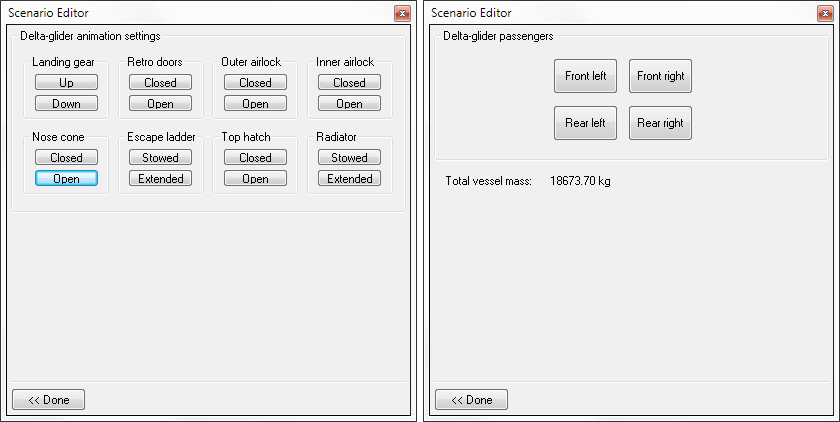
\includegraphics[width=\hsize]{dg_scneditor.png}
  \caption{DG animation control page (left) and passenger management page (right).}
\end{figure}


\subsubsection{Technical specifications}
Some design and operational parameters of the DG and DG-S spacecraft classes:

%\begin{table}[H]
	%\centering
	\begin{longtable}{ |p{0.4\textwidth}|p{0.2\textwidth}|p{0.2\textwidth}|p{0.05\textwidth}| }
	\hline\rule{0pt}{2ex}
	& \textbf{DG} & \textbf{DG-S} &\\
	\hline\rule{0pt}{2ex}
	Mass (empty) & 11.0 x 10$^{3}$ & 13.0 x 10$^{3}$ & kg\\
	\hline\rule{0pt}{2ex}
	Main tank capacity & 12.9 x 10$^{3}$ & 10.4 x 10$^{3}$ & kg\\
	\hline\rule{0pt}{2ex}
	Scram tank capacity & - & 2.5 x 10$^{3}$ & kg\\
	\hline\rule{0pt}{2ex}
	RCS tank capacity & 0.6 x 10$^{3}$ & 0.6 x 10$^{3}$ & kg\\
	\hline\rule{0pt}{2ex}
	Mass (payload) & 340 & 340 & kg\\
	\hline\rule{0pt}{2ex}
	Mass (total) & 24.84 x 10$^{3}$ & 26.84 x 10$^{3}$ & kg\\
	\hline\rule{0pt}{2ex}
	Thrust (main) & 2 x 160 & 2 x 160 & kN\\
	\hline\rule{0pt}{2ex}
	Thrust (retro) & 2 x 34 & 2 x 34 & kN\\
	\hline\rule{0pt}{2ex}
	Thrust (hover) & 110 + 2 x 36.3 & 110 + 2 x 36.3 & kN\\
	\hline\rule{0pt}{2ex}
	Thrust (scram, max) & - & 2 x 325 & kN\\
	\hline\rule{0pt}{2ex}
	Acceleration (main, max load) & 12.9 & 11.9 & m/s$^{2}$\\
	\hline\rule{0pt}{2ex}
	Acceleration (scram, max load) & - & 24.2 & m/s$^{2}$\\
	\hline\rule{0pt}{2ex}
	Isp (main, vacuum) & 4.0 x 10$^{4}$ & 4.0 x 10$^{4}$ & m/s\\
	\hline\rule{0pt}{2ex}
	Prop. flow rate (main, max) & 2 x 4.0 & 2 x 4.0 & kg/s\\
	\hline\rule{0pt}{2ex}
	Prop. flow rate (scram, max) & - & 2 x 3.0 & kg/s\\
	\hline\rule{0pt}{2ex}
	Dimensions (L x W x H) & 18.7 x 17.9 x 4.9 & 18.7 x 17.9 x 4.9 & m\\
	\hline\rule{0pt}{2ex}
	Inertia (PMI, mass-normalised, x, y, z) & 15.5, 22.1, 7.7 & 15.5, 22.1, 7.7 & m$^{2}$\\
	\hline\rule{0pt}{2ex}
	Stall C$_{L}$ & 1.0 & 1.0 &\\
	\hline\rule{0pt}{2ex}
	Stall AOA & 20 & 20 & deg\\
	\hline
	\end{longtable}
%\end{table}



\subsection{Shuttle-A}

\begin{figure}[H]
  \centering
  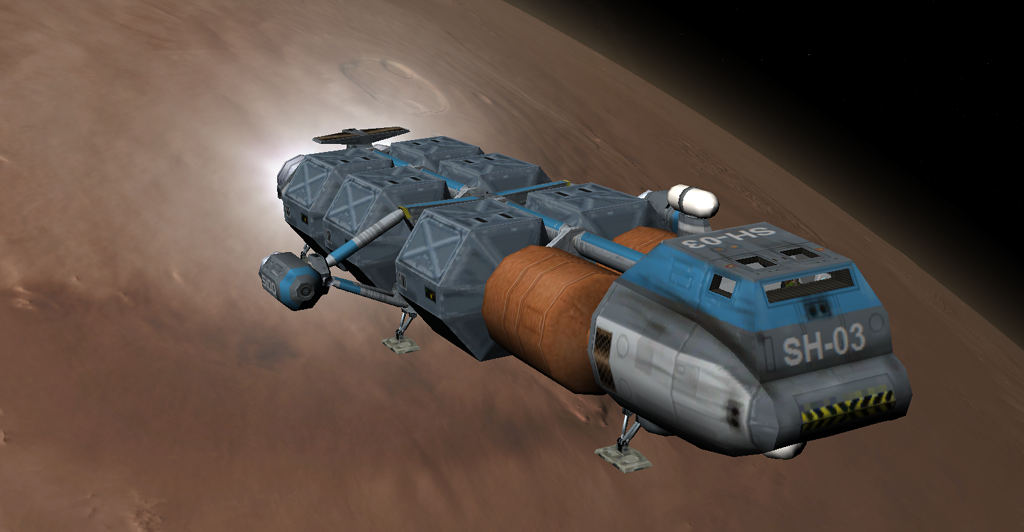
\includegraphics[width=\hsize]{shuttlea.png}
  \caption{Shuttle-A model design: Roger Long. Instrument panels and module code: Martin Schweiger. Virtual cockpit, payload management extensions: Radu Poenaru.}
\end{figure}

\noindent
The Shuttle-A class is a cargo vessel designed for a low gravity/low pressure operational environment. Its primary area of deployment is for transport duty between LEO (low Earth orbit), the Moon, Mars and and potentially moons in the outer solar system. In its current configuration it is also capable of achieving orbit from Earth's surface, but this requires a precise ascent profile.\\
The engine layout consists of a set of two main engines, two hover engines, and two engines in central side pods which can be rotated around 180° for retro thrust or to assist the main or hover engines.\\
The Shuttle-A contains a docking port and airlock below the habitat module which is protected by a hatch during atmospheric flight.\\
The avionics systems include, besides two standard MFD instruments, also a configurable attitude director indicator (ADI) for navigation.

\subsubsection{Instrument panels}
Cockpit views can be cycled with \keystroke{F8} between generic glass cockpit, 2-D panel and virtual cockpit modes. The virtual cockpit implementation for the Shuttle-A is currently quite rudimentary. The main avionics interface is provided with the 2-D cockpit mode.

\begin{figure}[H]
  \centering
  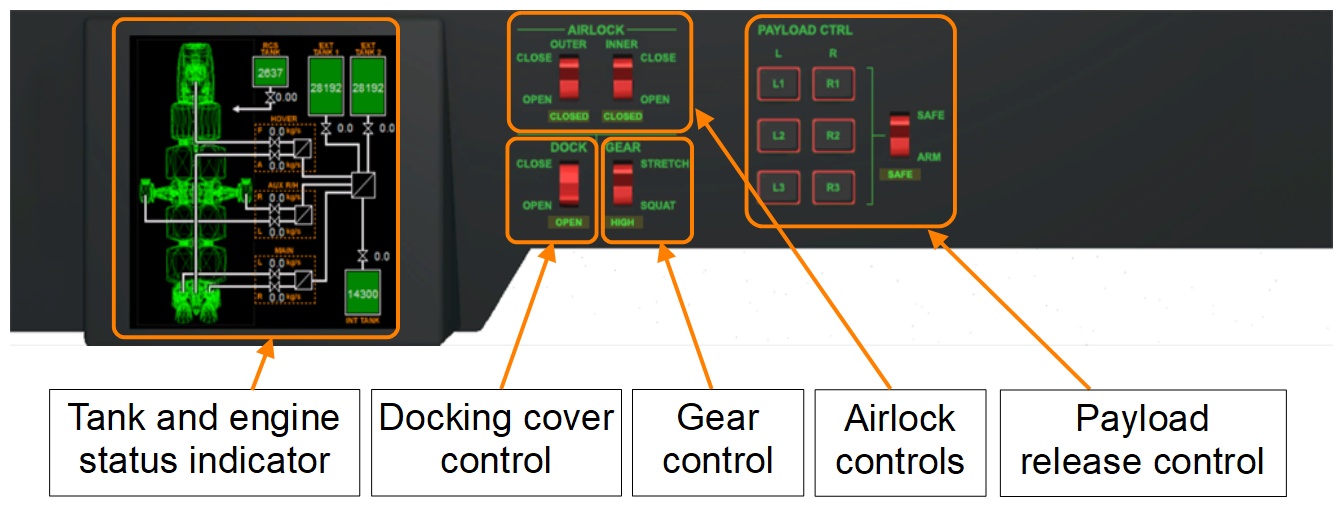
\includegraphics[width=\hsize]{shuttlea_panel1.png}
\end{figure}

\begin{figure}[H]
  \centering
  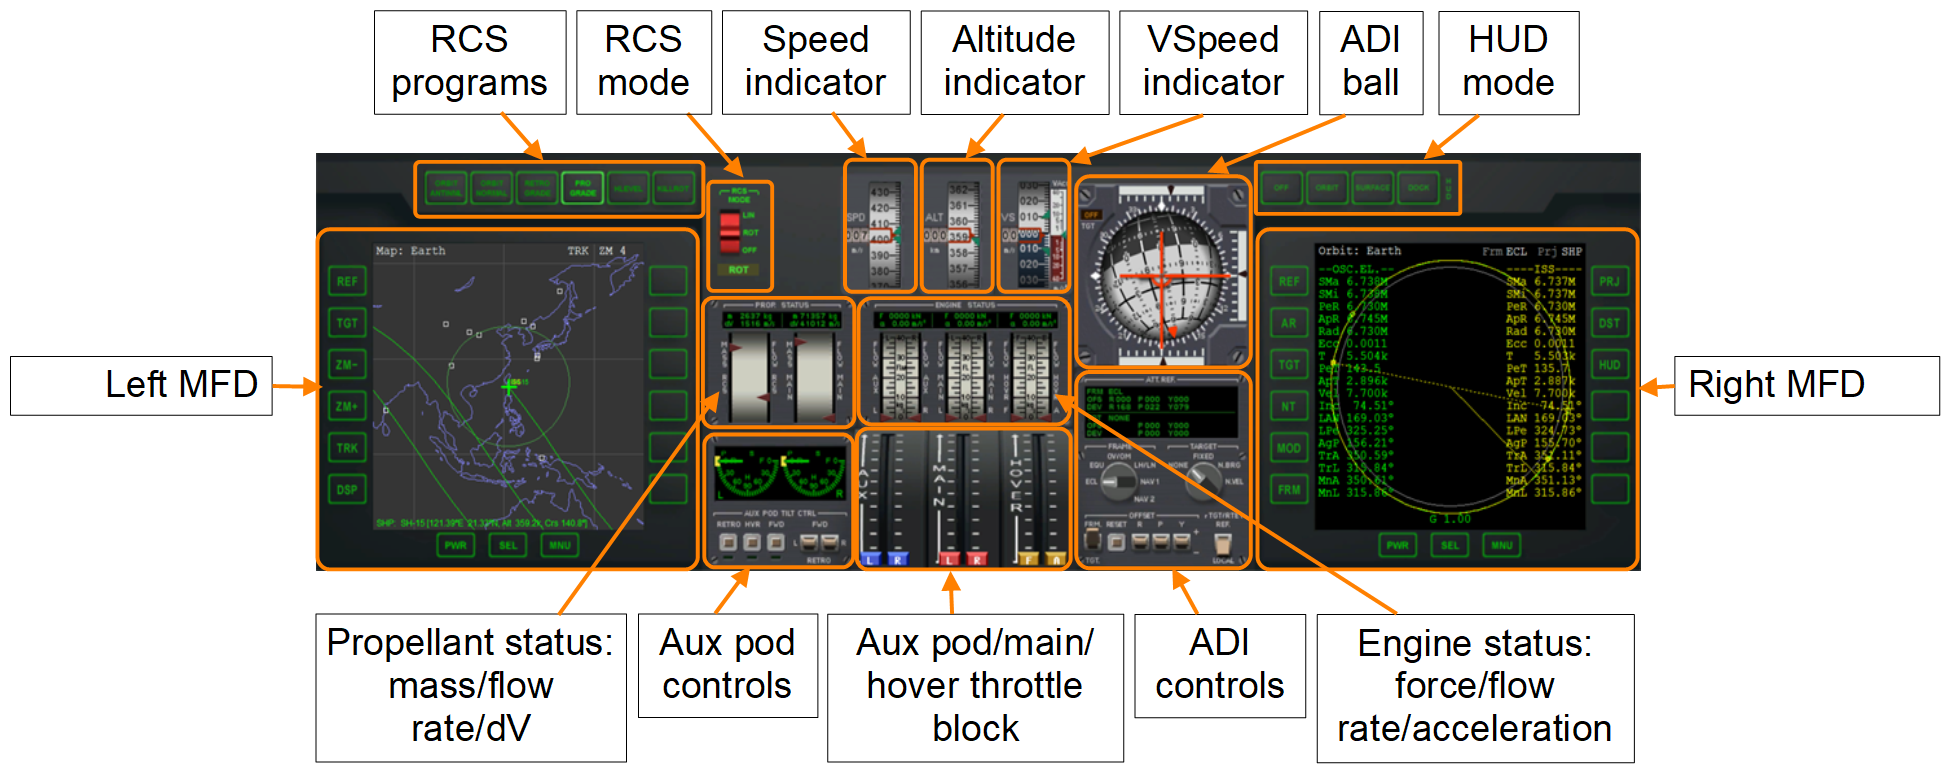
\includegraphics[width=\hsize]{shuttlea_panel0.png}
\end{figure}

\paragraph{Main panel}
%TODO add section link
The 2-D cockpit view consists of main and overhead panels. They can be switched between with \Ctrl\UArrow and \Ctrl\DArrow. The main panel contains the primary avionics instruments - left and right MFD (see TODO for standard MFD modes), ADI ball and controls (see TODO) and speed, altitude and vertical speed readouts.\\
The engine block is located in the bottom centre of the panel. Main, hover and auxiliary thrusters can be operated individually, by engaging the throttle controls separately, or in pairs, by clicking and dragging between throttle sliders.\\
%TODO add section link
Left of the throttle block is the auxiliary pod control panel which can be used to rotate the pods and has readouts for current orientation (see TODO).\\
Above the throttle block are readouts for tank and engine status, including fuel mass, delta-V estimates, thrust force and acceleration, and fuel flow rates.\\
At the top centre of the panel are located tape indicators for speed, vertical speed and altitude. At the left are the controls for RCS mode and programs, at the right is the HUD mode selector.

\paragraph{Attitude reference and ADI}
The attitude director indicator (ADI) provides feedback to the pilot about the spacecraft orientation with respect to a given frame of reference. It consists of a ball that can rotate and is always aligned with the reference frame, and a direction index representing the orientation of the spacecraft (given its pitch, yaw and roll angles) relative to the frame.

\begin{figure}[H]
  \centering
  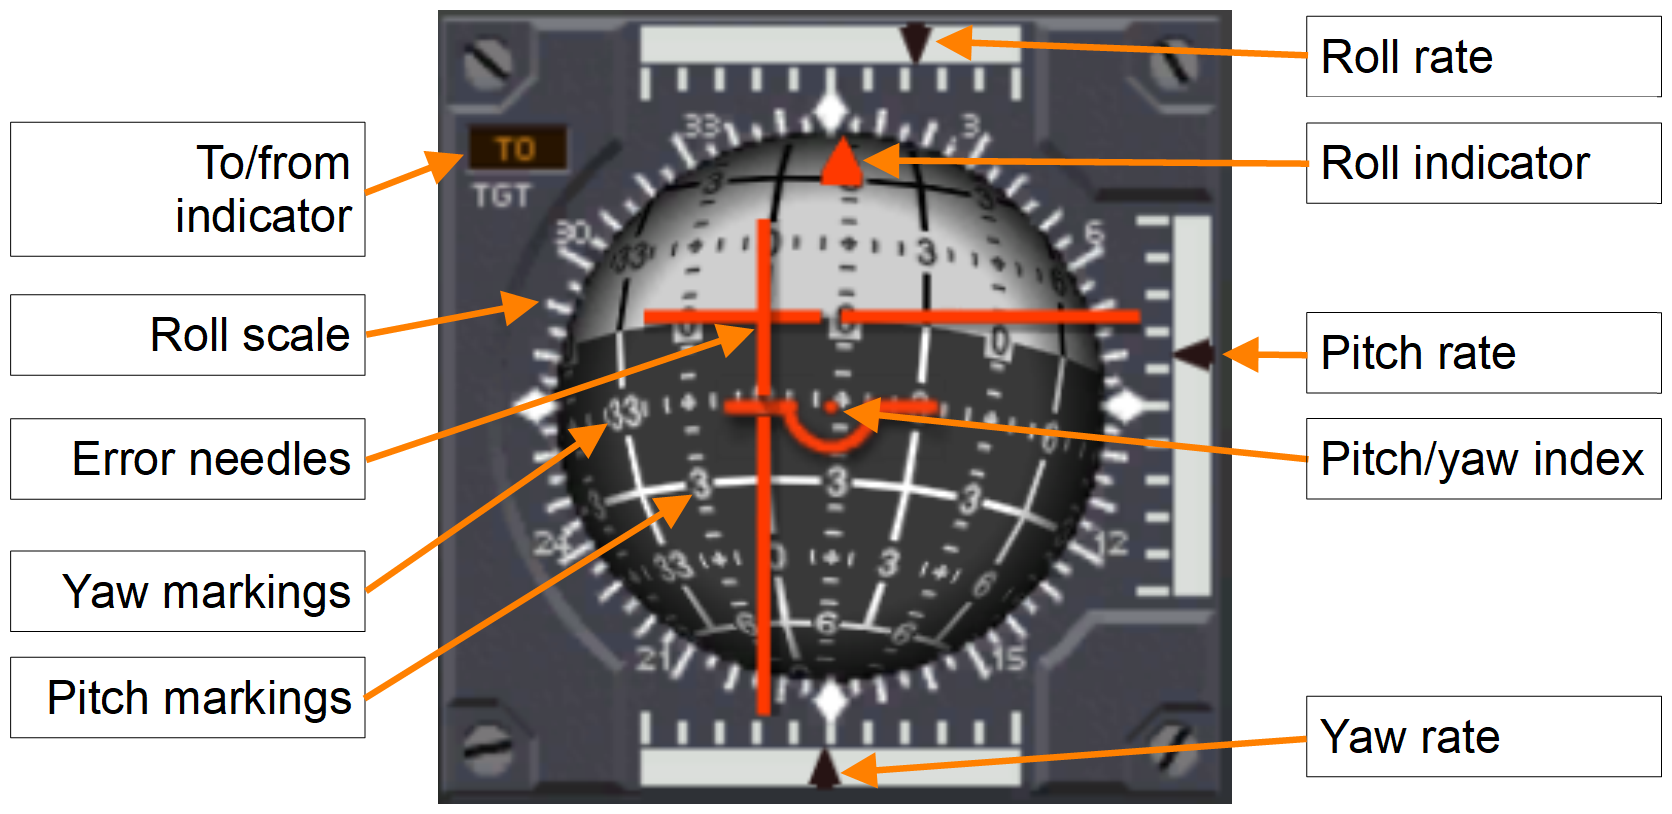
\includegraphics[width=0.9\hsize]{shuttlea_adi_ball.png}
\end{figure}

\noindent
The parameters of the attitude reference, as well as the operation mode of the ADI, can be controlled by the panel below the ADI.

\begin{figure}[H]
  \centering
  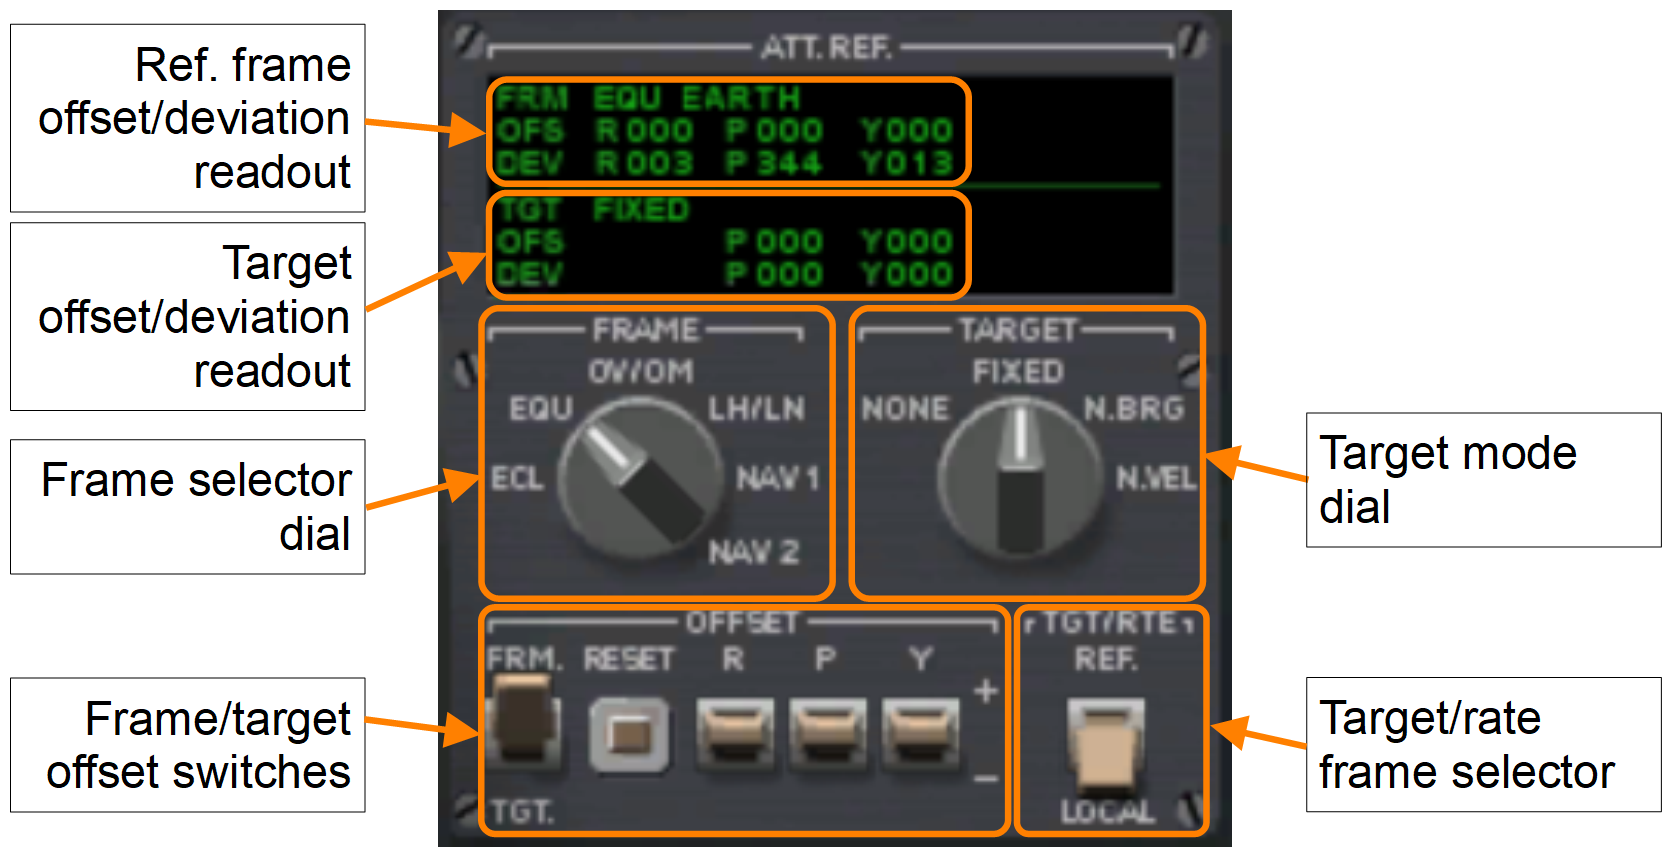
\includegraphics[width=0.9\hsize]{shuttlea_adi_ctrl.png}
\end{figure}

\noindent
\textbf{Attitude frame}\\
The frame selection dial sets the reference frame represented by the ADI. In practice, the most useful reference frame will depend on the current task or journey segment.

\begin{itemize} 
\item \textbf{Ecliptic (ECL).} Reference frame is the ecliptic and equinox of epoch J2000.0. Direction (P=0, Y=0) is aligned with the vernal point. Direction (P=+90) points to the ecliptic north pole. This inertial frame is most useful for interplanetary trips.
\item \textbf{Equator (EQU).} Reference frame is the equator of the body currently being orbited. Direction (P=0, Y=0) points to the ascending node of the ecliptic w.r.t. the planet's equator. Direction (P=+90) points in the positive direction of the planet's rotation axis. This is a (nearly) inertial frame (subject to the planet's axis precession), and most useful for orbital operations.
\item \textbf{Orbital velocity/Orbital momentum vector (OV/OM).} This is a rotating frame. The axis (P=0, Y=0) is aligned with the vessel's current orbital velocity vector relative to the orbit reference body. The (P=+90) axis is aligned with the orbital momentum vector (i.e. perpendicular to the orbital plane). This reference frame is equivalent to that used by the Orbit HUD mode, but rotated by 90° in roll.
\item \textbf{Local horizon/Local north (LH/LN).} This is a rotating frame. The axis (P=0, Y=0) is aligned with the local heading = 0 direction in the local horizon plane. Axis (P=+90) is aligned with the normal of the local horizon plane. This reference frame is equivalent to that used by the Surface HUD mode.
\item \textbf{Link to NAV radio source (NAV 1/2).} The reference frame can be selected implicitly by feeding data from one of the NAV radio receivers to the ADI. The orientation of the frame depends on the NAV signal type. Currently supported is IDS (instrument docking system) input, which aligns the ADI reference with the docking port orientation: Direction (P=0, Y=0) is aligned with the approach direction; (P=+90) is aligned with the "Up" direction for longitudinal rotation alignment.
\end{itemize}

\noindent
A user-defined offset can be added to any of the predefined reference frames. To do this, set the selector toggle in the "Offset" group to "Frm", and then use the "R" (roll), "P" (pitch) and "Y" (yaw) switches to add an offset to any of the three Euler angles. The "Reset" button resets the offsets to zero.\\
\\
\textbf{Target}\\
The ADI contains two error needles designating the direction of a target on top of the ADI ball. The needles form a cross-hair marking a particular point on the ADI ball (within the limit of about +/- 40° in pitch and yaw from the current vessel orientation). The type of target can be selected with the "Target" dial on the control panel.


\begin{itemize} 
\item \textbf{None (no target).} The error needles are deactivated and return to the centered position. Target indicator on the ADI instrument shows "OFF".
\item \textbf{Fixed (fixed location relative to reference frame).} In this mode, the error needles mark a fixed point on the ADI ball. By default, this is the point (P=0, Y=0), but any pitch/yaw direction can be selected by specifying target offsets (see below).
\item \textbf{N. Brg (NAV transmitter bearing).} If the reference frame is set to NAV 1 or 2, and the specified NAV receiver is currently tuned to a transmitter in range, the error needles point to the bearing of the transmitter in the current frame. Otherwise the error needles are deactivated.
\item \textbf{N. Vel (NAV transmitter velocity).} If the reference frame is set to NAV 1 or 2, and the specified NAV receiver is currently tuned to a transmitter in range, the error needles point to the velocity of the transmitter relative to the spacecraft. Otherwise the error needles are deactivated.
\end{itemize}

\noindent
Note that in all modes, the error needles mark the direction 180° away from the target as well as the direction towards the target. To distinguish between the two, the ADI ball shows "TO" and "FROM" in the target indicator box. For example, if the target is set to N. Brg, the needles are centered, and the target indicator shows "FROM", the target is located exactly behind the spacecraft.\\
Similar to the reference frame, an offset can be added to the target direction. To do this, set the selector toggle in the Offset group to "TGT" and use the "P" (pitch) and "Y" (yaw) switches to define an offset. Note that the "R" (roll) switch is not used for target offsets. The "Reset" button resets the target offsets to zero.\\
\\
\textbf{Attitude rates}\\
The rates of change in pitch, yaw and roll are displayed by indicators at the left, bottom and top edge of the instrument, respectively. The indicator ranges are -10°/s to +10°/s for all three angles, with tick marks spaced at 2°/s. The rates can be displayed either in the local vessel frame or the reference frame. Use the "TGT/RTE" switch to select the mode.\\
\\
\textbf{ADI layout}\\
The ADI ball is available in two layouts:

%\begin{table}[H]
	%\centering
	\begin{longtable}{ |p{0.15\textwidth}|p{0.25\textwidth}|p{0.25\textwidth}|p{0.25\textwidth}| }
	\hline\rule{0pt}{2ex}
	\textbf{Layout} & \textbf{Pitch range} & \textbf{Yaw range} & \textbf{Poles}\\
	\hline\rule{0pt}{2ex}
	0 & -90° - +90° & 0° - 360° & at pitch = -90° and +90°\\
	\hline\rule{0pt}{2ex}
	1 & 0° - 360° & -90° - +90° & at yaw = -90° and +90°\\
	\hline
	\end{longtable}
%\end{table}

\noindent
The layout can be selected on a per vessel/per scenario basis by adding an ADI\_LAYOUT item with value 0 or 1 to the Shuttle's scenario entry. If this item is not present, the value in the ShuttleA configuration file (.\textbackslash Config\textbackslash Vessels\textbackslash ShuttleA.cfg) is used. If this entry is also not present, layout 0 is assumed. The layout can be switched interactively in the running simulation from a console with the command

\begin{lstlisting}[language=OSFS]
v:set_adilayout(layout)
\end{lstlisting}

\noindent
where v is an interface instance to Shuttle-A vessel and \textit{layout} is 0 or 1.\\
Note that the two layouts don't alter the behaviour of the ADI ball, just the markings painted on it. They do however represent different attitude angle interpretations, i.e. the Euler angles differ between the two layouts.
The Tutorials\textbackslash ADI training scenario is an interactive tutorial that demonstrates the ADI concept and operation directly in Orbiter. Try it!


\paragraph{Auxiliary pod control}
The two auxiliary engine pods mounted at the central rib of the Shuttle-A's payload spine can be rotated  around the transversal axis by 180° to point the installed engines either aft (to assist with main thrust), downward (to assist with hover thrust), forward (to provide retro thrust) or at any intermediate position. The pod rotation controls are located left of the throttle block.

\begin{figure}[H]
  \centering
  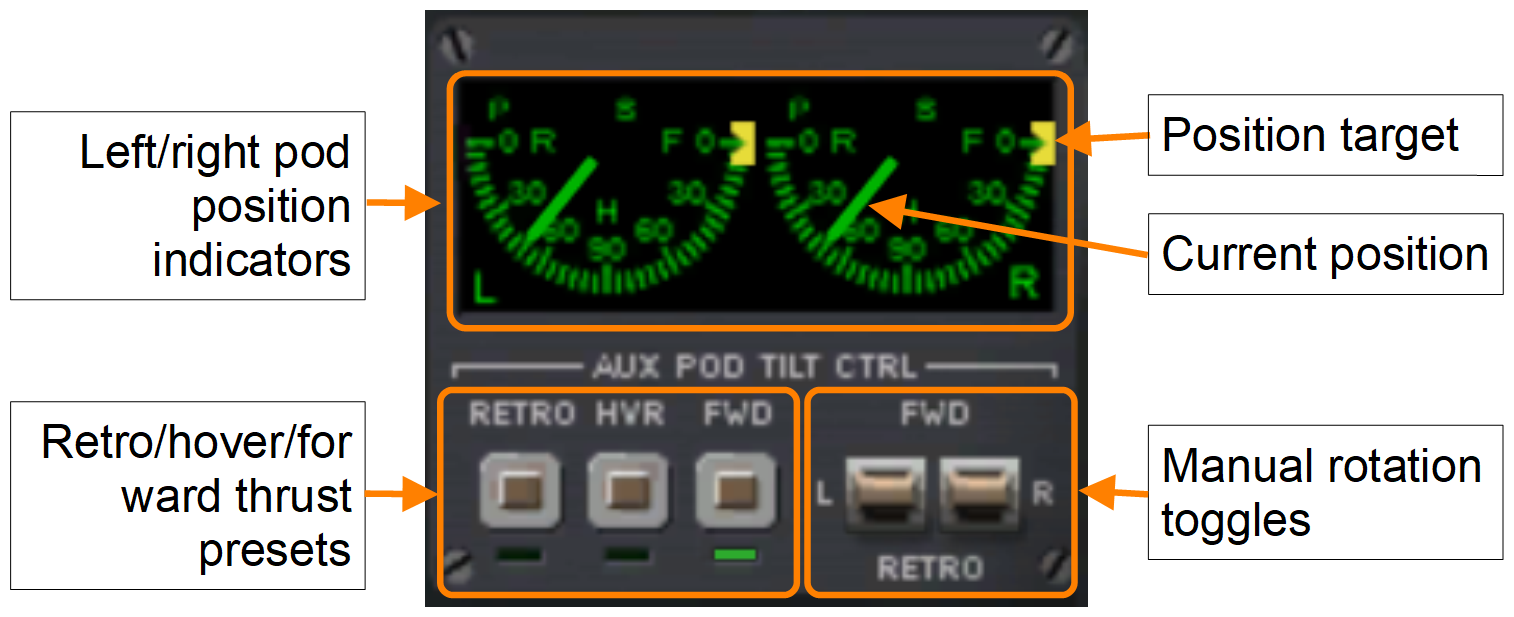
\includegraphics[width=0.9\hsize]{shuttlea_pod_ctrl.png}
\end{figure}

\noindent
The two displays at the top show the left and right pods' current positions (green hands) and commanded target positions (yellow bugs). The pods' rotation speed is finite (approximately 23°/s), so the actual position will lag behind the commanded values. The R-0 position represents the engines pointing forward (retro thrust); the F-0 position represents the engines point aft (forward thrust), and the H-90 position represents the engines pointing downward (hover thrust).\\
The AUX POD TILT CTRL block below the displays contains the controls for rotating the pods. The three buttons to the left command presets for the R-0 position (RETRO), H-90 (HVR) and F-0 (FWD) for both pods. The two toggle switches to the right enable manual adjustments towards the forward thrust (FWD) or retro thrust direction (RETRO). The commands can either be issued to a single pod by activating only one of the toggles, or to both pods simultaneously by clicking between the toggles.\\
When launching a fully loaded Shuttle-A from Earth's surface, the auxiliary pods must be engaged in hover position together with the regular hover engines to achieve lift-off. As the vessel gains altitude, the main engines are engaged and the ship pitches up using RCS. The auxiliary pods will be gradually rotated backward toward the F-0 position to provide additional main thrust, while the hover engines are throttled down.


\begin{figure}[H]
  \centering
  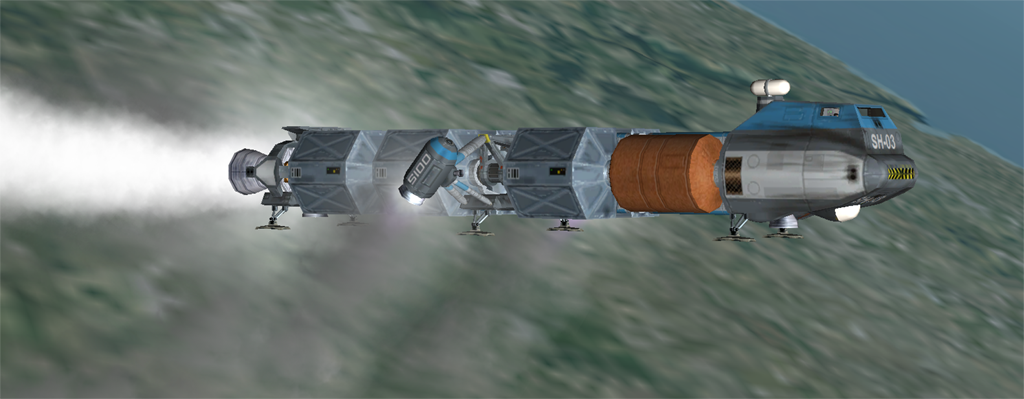
\includegraphics[width=\hsize]{shuttlea_auxpods.png}
  \caption{Shuttle-A at launch with auxiliary pods transitioning from hover to aft position.}
\end{figure}

\paragraph{Overhead panel}
The overhead panel contains a display for tank and engine status. It has readouts for current tank fill status and mass flow rates for the main fuel pumps.~\\
The panel also contains controls for operating the docking covers, gear struts and outer/inner airlock hatches.\\
Located on the right side of the panel are the controls for releasing the six cargo containers the Shuttle-A can carry. To release a cargo container, first arm the release mechanism (main control switch from SAFE to ARM). Then click on a container position (L/R 1-3) to release it. Empty payload positions are marked with a red border. When done, return the main control switch back to SAFE.\\
Containers can be released on the ground or during flight. On the ground, make sure to move the landing gear struts to "squatting" position to set the containers down gently. You can drop containers while in low-level flight over a planetary surface (don't drop them from high altitude or at high speed to avoid damaging them or your ship), or during orbital operations. If releasing in weightless conditions (in orbit), use RCS to move away from the released container (up or down in linear RCS mode).

\subsubsection{Keyboard controls}
In addition to the generic Orbiter vessel control keys, the Shuttle-A supports the following vessel-specific key controls:
%\begin{table}[H]
	%\centering
	\begin{longtable}{ |p{0.2\textwidth}|p{0.7\textwidth}| }
	\hline\rule{0pt}{2ex}
	\textbf{Shortcut} & \textbf{Action}\\
	\hline\rule{0pt}{2ex}
	\keystroke{G} & Operate landing gear struts between "stretch" and "squat" positions.\\
	\hline\rule{0pt}{2ex}
	\keystroke{K} & Operate the docking cover mechanism.\\
	\hline\rule{0pt}{2ex}
	\keystroke{O} & Operate the outer airlock hatch.\\
	\hline\rule{0pt}{2ex}
	\Ctrl\keystroke{O} & Operate the inner airlock hatch.\\
	\hline\rule{0pt}{2ex}
	\Ctrl\keystroke{0}$_{Num}$ & Increase auxiliary pod engine thrust.\\
	\hline\rule{0pt}{2ex}
	\Ctrl\keystroke{.}$_{Num}$ & Decrease auxiliary pod engine thrust.\\
	\hline
	\end{longtable}
%\end{table}

\subsubsection{Technical specifications}
Some design and operational parameters of the Shuttle-A spacecraft class:

%\begin{table}[H]
	%\centering
	\begin{longtable}{ |p{0.45\textwidth}|p{0.3\textwidth}|p{0.15\textwidth}| }
	\hline\rule{0pt}{2ex}
	Mass (empty) & 13.0 $\cdot$ 10$^{3}$ & kg\\
	\hline\rule{0pt}{2ex}
	Main tank capacity & 71.5 $\cdot$ 10$^{3}$ & kg\\
	\hline\rule{0pt}{2ex}
	RCS tank capacity & 2.7 $\cdot$ 10$^{3}$ & kg\\
	\hline\rule{0pt}{2ex}
	Mass (payload, max.) & 6 x 20.0 $\cdot$ 10$^{3}$ & kg\\
	\hline\rule{0pt}{2ex}
	Mass (total, max.) & 207.2 $\cdot$ 10$^{3}$ & kg\\
	\hline\rule{0pt}{2ex}
	Thrust (main) & 2 x 1064.4 & kN\\
	\hline\rule{0pt}{2ex}
	Thrust (hover) & 2 x 745.0 & kN\\
	\hline\rule{0pt}{2ex}
	Thrust (aux. pods) & 2 x 385.0 & kN\\
	\hline\rule{0pt}{2ex}
	Thrust (RCS, linear mode) & 2 x 4.5 & kN\\
	\hline\rule{0pt}{2ex}
	Torque (RCS pitch, yaw) & 2 x 67.5 & kNm\\
	\hline\rule{0pt}{2ex}
	Torque (RCS roll) & 2 x 27.1 & kNm\\
	\hline\rule{0pt}{2ex}
	Acceleration (main + aux, max. load) & 14.0 & m/s$^{2}$\\
	\hline\rule{0pt}{2ex}
	Acceleration (hover + aux, max. load) & 10.9 & m/s$^{2}$\\
	\hline\rule{0pt}{2ex}
	Isp (main, vacuum) & 3.3 $\cdot$ 10$^{4}$ & m/s\\
	\hline\rule{0pt}{2ex}
	Prop. flow rate (main, max.) & 2 x 32.3 & kg/s\\
	\hline\rule{0pt}{2ex}
	Dimensions (L x W x H) & 35.0 x 15.4 x 6.9 & m\\
	\hline\rule{0pt}{2ex}
	Inertia (PMI, mass-normalised) & 86.6 (xx), 89.8 (yy), 5.5 (zz) & m$^{2}$\\
	\hline\rule{0pt}{2ex}
	Docking port, reference position & (0, 0, 18.7) & m\\
	\hline\rule{0pt}{2ex}
	Docking port, approach direction & (0, 0, 1) & \\
	\hline
	\end{longtable}
%\end{table}


\subsubsection{Credits}
Special thanks to Roger "Frying Tiger" Long for his excellent model of the Shuttle-A, and to Radu Poenaru for the virtual cockpit implementation and code extensions, including cargo management and landing gear.


\subsection{Shuttle PB (PTV)}
The PB is a very agile single-seat spacecraft. It has a main engine and uses hover thrusters for vertical take-off and landing. During atmospheric flight the lifting body and winglets produces lift. However, aerodynamic control surfaces are not supported in the current version. Attitude control is performed via the reaction control system (RCS).\\

\begin{figure}[H]
  \centering
  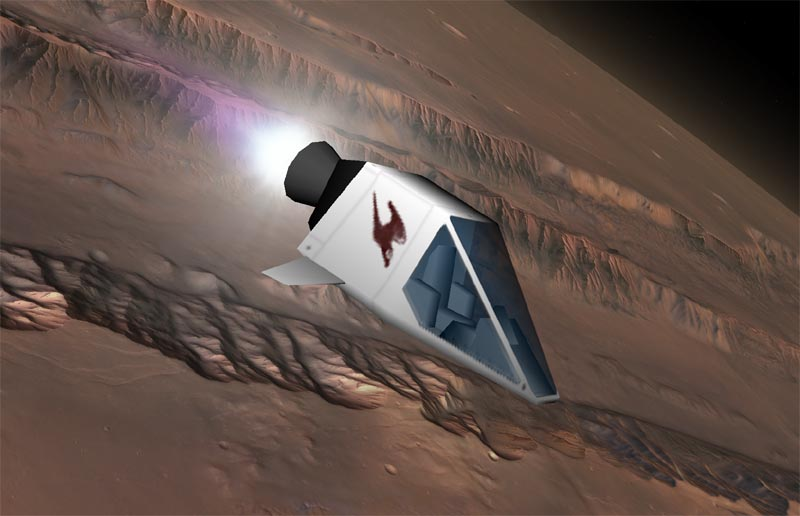
\includegraphics[width=0.75\hsize]{shuttle_pb.jpg}
  \caption{Overall design and textures: Balázs Patyi. Model improvements: Martin Schweiger}
\end{figure}

\noindent
%TODO add section link
Apart from the standard implementation of the PB vessel class, Orbiter also comes with a script version of this spacecraft type (\textit{ScriptPB}). This looks and behaves identical to the original Shuttle PB, but is completely implemented as a Lua script (see chapter TODO) and can therefore easily be modified. This is a good way for newcomers to get into spacecraft design. The code can be found in Config\textbackslash ScriptPB.cfg.\\
\\
\textbf{Technical specifications:}

%\begin{table}[H]
	%\centering
	\begin{longtable}{ |p{0.25\textwidth}|p{0.15\textwidth}|p{0.05\textwidth}|p{0.45\textwidth}| }
	\hline\rule{0pt}{2ex}
	Mass & 500 & kg & (empty)\\
	\hline\rule{0pt}{2ex}
	& 750 & kg & (fuel capacity)\\
	\hline\rule{0pt}{2ex}
	& 1250 & kg & (total)\\
	\hline\rule{0pt}{2ex}
	Dimensions & 6.8 x 5.2 x 2.4 & m & (L x W x H)\\
	\hline\rule{0pt}{2ex}
	Thrust & 30.0 & kN & (main)\\
	\hline\rule{0pt}{2ex}
	& 2 x 7.5 & kN & (hover)\\
	\hline\rule{0pt}{2ex}
	Acceleration & 24.0 & m/s$^{2}$ & (main thrust at full load)\\
	\hline\rule{0pt}{2ex}
	Isp & 5.0 $\cdot$ 10$^{4}$ & m/s & (vacuum)\\
	\hline
	\end{longtable}
%\end{table}



\subsection{Dragonfly}
The Dragonfly is a space tug designed for moving payload in orbit. It may be used to bring satellites delivered by the Space Shuttle into higher orbits, or to help in the assembly of large orbital structures.

\begin{figure}[H]
  \centering
  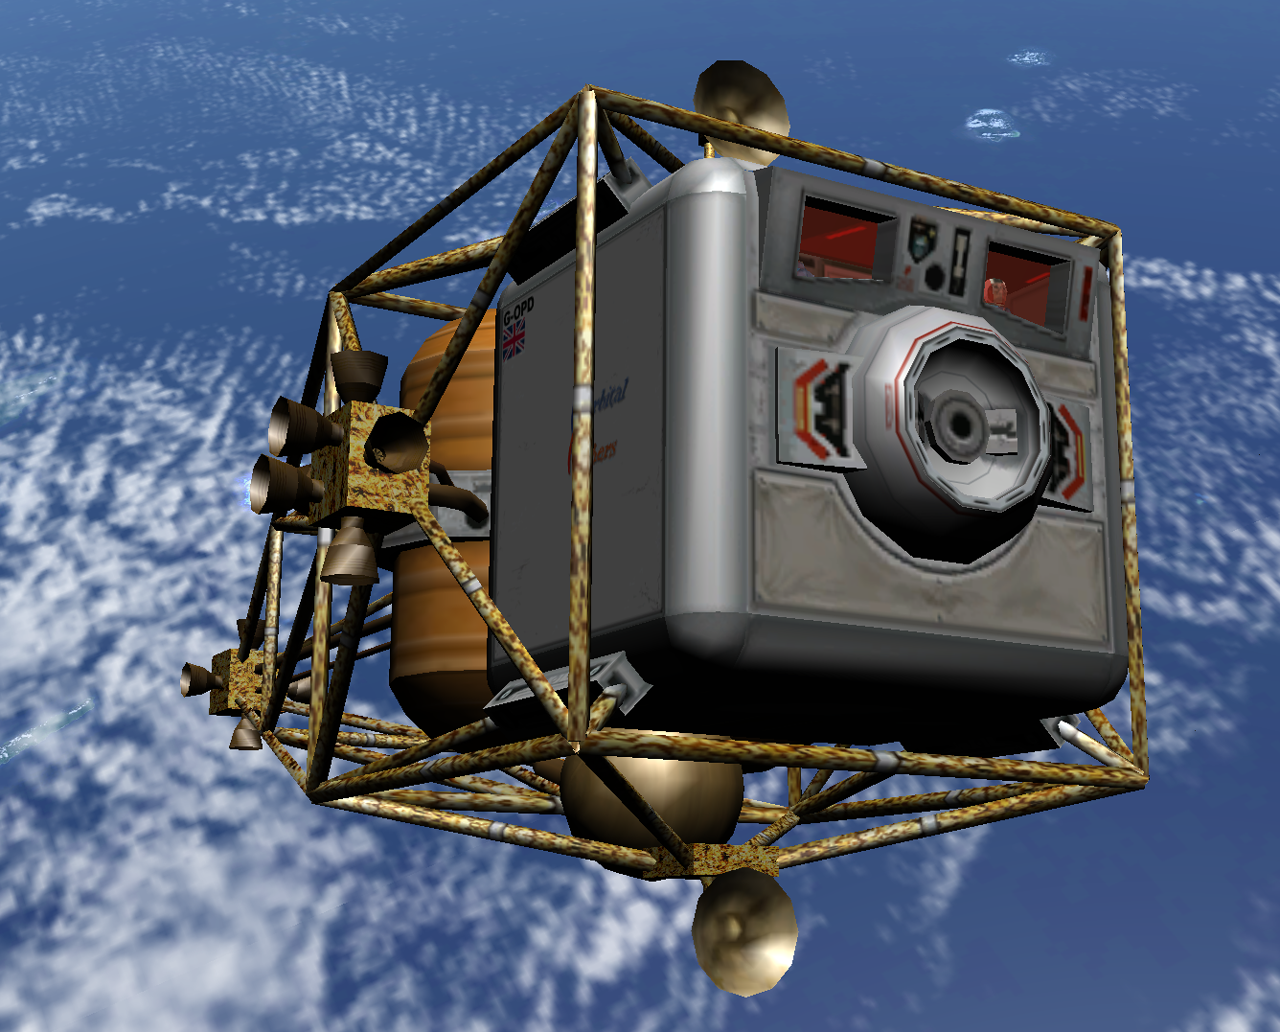
\includegraphics[width=0.75\hsize]{dragonfly.png}
  \caption{Dragonfly original design: Martin Schweiger. Model improvements and textures: Roger Long. Systems simulation and instrument panels: Radu Poenaru.}
\end{figure}

\noindent
The Dragonfly has no dedicated main engines, but a versatile and adjustable reaction control system for manoeuvring. It is not designed for atmospheric descent or surface landing.\\
The cockpit layout consists of a set of 2D panels that include MFD instruments, an ADI ball and radar display. The Dragonfly incorporates a detailed electrical and environmental systems simulation, contributed by Radu Poenaru.

%\begin{table}[H]
	%\centering
	\begin{longtable}{ |p{0.25\textwidth}|p{0.15\textwidth}|p{0.05\textwidth}|p{0.45\textwidth}| }
	\hline\rule{0pt}{2ex}
	Mass & 7.0 $\cdot$ 10$^{3}$ & kg & (empty)\\
	\hline\rule{0pt}{2ex}
	& 4.0 $\cdot$ 10$^{3}$ & kg & (fuel capacity)\\
	\hline\rule{0pt}{2ex}
	& 11.0 $\cdot$ 10$^{3}$ & kg & (total)\\
	\hline\rule{0pt}{2ex}
	Dimensions & 14.8 x 7.2 x 7.4 & m & (L x W x H)\\
	\hline
	\multicolumn{4}{|c|}{\rule{0pt}{2ex}Propulsion system: RCS with thrusters mounted in 3 pods (left, right, aft)}\\
	\hline\rule{0pt}{2ex}
	Thrust & 1.0 & kN & (per RCS engine)\\
	\hline\rule{0pt}{2ex}
	Acceleration & 0.18 & m/s2 & (linear RCS engine pair thrust, at full load)\\
	\hline\rule{0pt}{2ex}
	Isp & 4.0 $\cdot$ 10$^{3}$ & m/s & (vacuum)\\
	\hline\rule{0pt}{2ex}
	Prop. flow rate & 0.50 & kg/s & (RCS engine pair in single axis)\\
	\hline
	\caption{Technical specifications}
	\end{longtable}
%\end{table}


\subsubsection{Electrical Power System}

\begin{figure}[H]
  \centering
  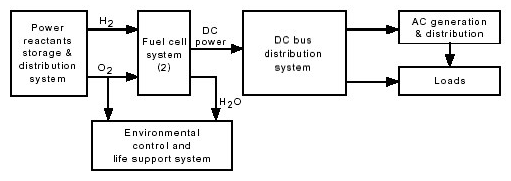
\includegraphics[width=0.75\hsize]{dragonfly_electricalsystem.png}
  \caption{Electrical Power System}
\end{figure}

\noindent
The electrical power system (EPS) consists of the equipment and reactants that produce electrical power for distribution throughout the space vehicle, and fulfill all power requirements of the vessel. The EPS operates during all flight phases. For nominal operations, very little flight crew interaction is required by the EPS. The vessel has no primary hydraulic system, and thus all operating and motor power is electrical-based.\\
The EPS is functionally divided into three subsystems: power reactants storage and distribution (PRSD), two fuel cell power plants (fuel cells) + one battery, and electrical power distribution and control (EPDC).\\
The two fuel cells generate all 28-volt direct-current electrical power for the vehicle through an electrochemical reaction of hydrogen and oxygen. At the hydrogen electrode (anode), hydrogen is oxidized according to the following reaction:

\begin{align*}
\ce{2H_{2} + 4OH^{-} -> 4H_{2}O + 4e^{-}}
\end{align*}

\noindent
forming water and releasing electrons. At the oxygen electrode (cathode), oxygen is reduced in the presence of water. It forms hydroxyl ions according to the following relationship:

\begin{align*}
\ce{O_{2} + 2H_{2}O -> 4OH^{-}}
\end{align*}

\noindent
The net reaction consumes one oxygen molecule and two hydrogen atoms in the production of two water molecules, with electricity and heat formed as by-products of the reaction.\\
The power reactants storage and distribution system stores the reactants (cryogenic hydrogen and oxygen) and supplies them to the two fuel cells that generate all the electrical power for the vehicle during all mission phases. In addition, the subsystem supplies cryogenic oxygen to the environmental control and life support system (ECLSS) for crew cabin pressurization. The hydrogen and oxygen are stored in three tanks each at cryogenic temperatures (170 K for liquid oxygen and 70 K for liquid hydrogen) and supercritical pressures (above 1400 kPa for oxygen and above 2000 kPa for hydrogen).\\
The system stores the reactant hydrogen and oxygen in double-walled, thermally insulated spherical tanks with a vacuum annulus between the inner pressure vessel and outer tank shell. Each tank has heaters to add energy to the reactants during depletion to control pressure. Each tank is capable of measuring quantity remaining.


\paragraph{Power Reactants Storage and Distribution (PRSD)}

\begin{figure}[H]
  \centering
  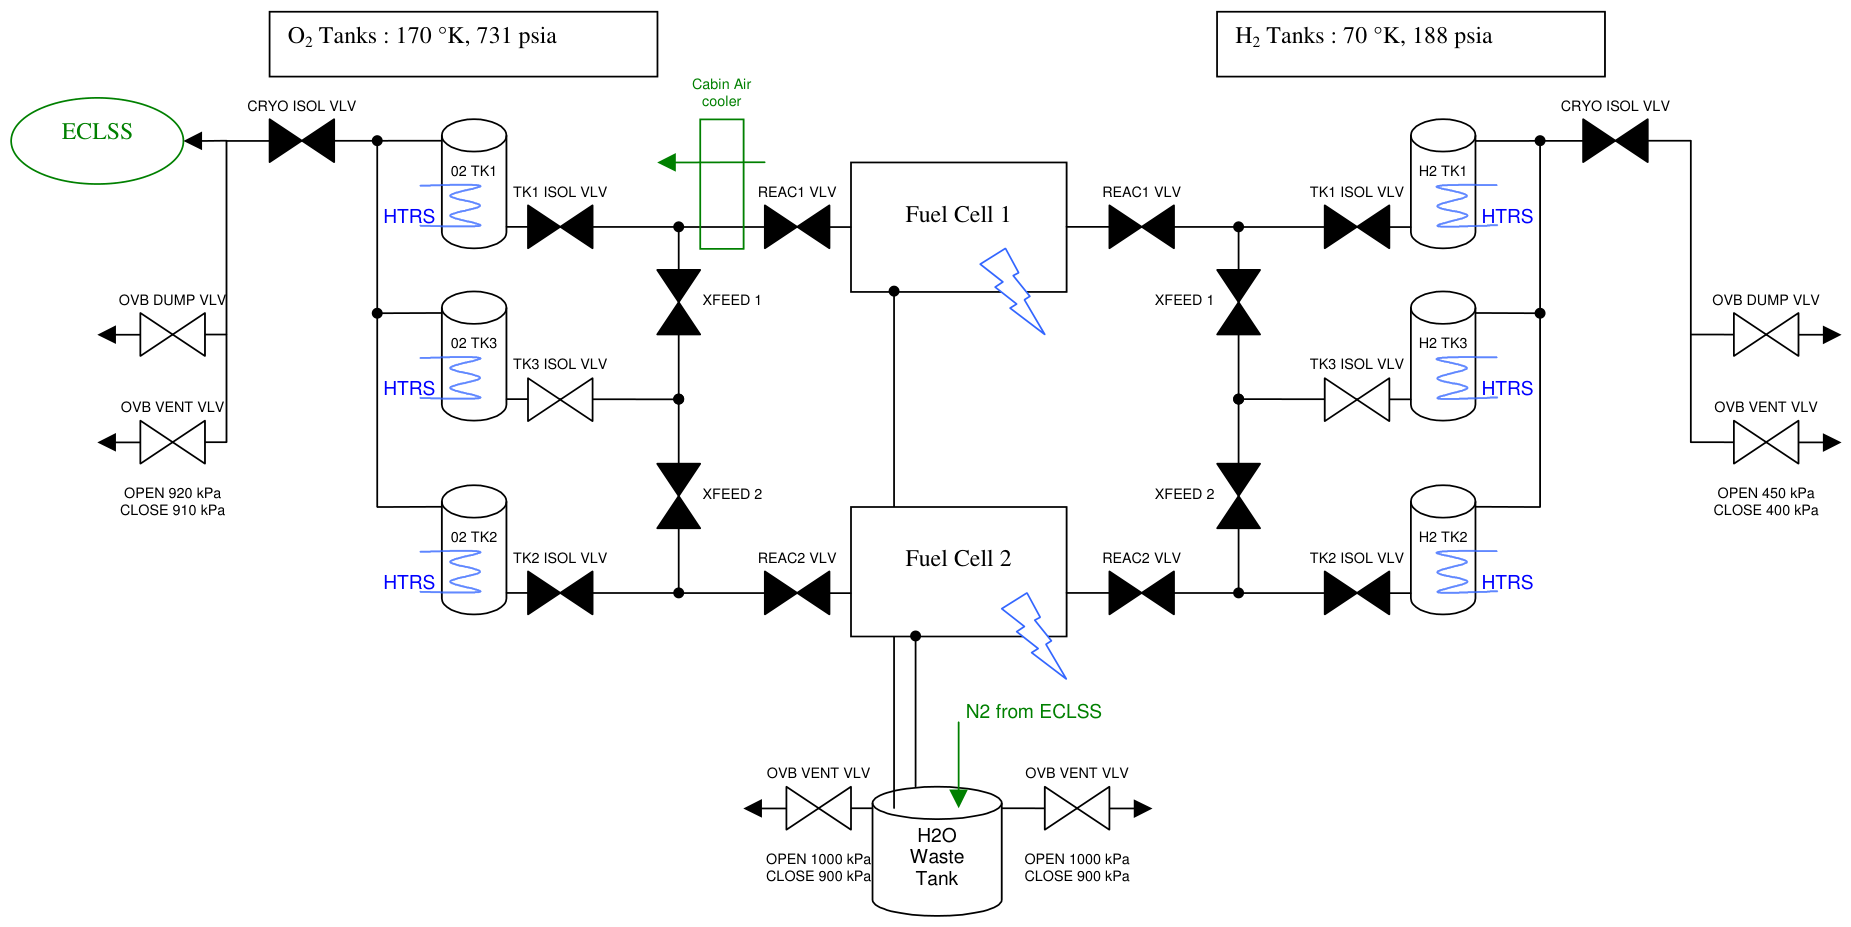
\includegraphics[width=\hsize]{dragonfly_diagram_prsd.png}
\end{figure}

\noindent
PRSD is controlled by switches located in the upper-left corner and lower-left corner of panel L1 (main electrical panel). The switches can direct the flow of cryogenic reactants and isolate parts of PRSD in case of leaks.

\begin{figure}[H]
  \centering
  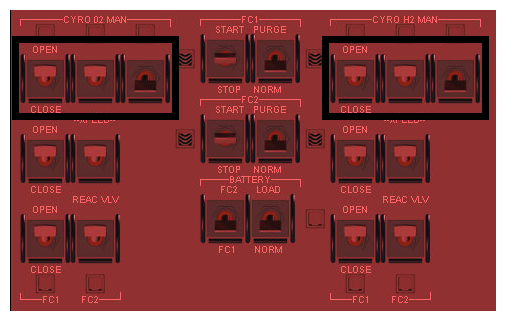
\includegraphics[width=0.5\hsize]{dragonfly_prsd_1.png}
\end{figure}

\noindent
The top row of switches control isolation valves for each of the three oxygen and hydrogen tanks (TK ISOL VLV). When set to close (down pos.) a DC powered engine will mechanically close reactant access to PRDS. Typical setting is tanks 1 and 2 open, tank 3 isolated. Isolation motor operation is indicated by a TB (talk-back) indicator above each switch. TB will show white when isol. motor is stopped and barberpole when motor is operating or is damaged.\\
Typical closing time for an isol. valve is about 3 seconds. Given that isol. valves operation is necessary in certain circumstances to start/restart the fuel cells, the power needed for motor operation is provided directly by the battery rather than from a DC bus. Care must be taken that a minimum power capacity is stored in the battery to assure isol. valve functioning in case of fuel-cell shutdown.

\begin{figure}[H]
  \centering
  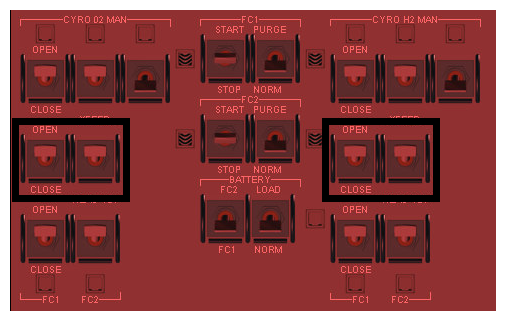
\includegraphics[width=0.5\hsize]{dragonfly_prsd_2.png}
\end{figure}

\noindent
Second row of switches controls cross-feed valves in the cryogenic manifold (XFEED). Normal piping configuration is tank 1 supplying reactant to FC1, tank 2 supplying reactant to FC2 and tank 3 functioning as back-up and ECLSS supply. By positioning the XFEED switch 1 to open, tanks 1and 3 will supply reactants to both FC1 and ECLSS.\\
Positioning the XFEED switch 2 to open, tanks 2 and 3 supply reactants to FC2 and ECLSS. Opening both XFEED valves, tanks 1, 2 and 3 supply reactants to FC1, FC2 and ECLSS.\\
Last two switches on the last row (REAC VLV) control the reactant valves to the respective fuel cells. Same operating procedures apply as for the tank isolation valves, with a closing time of $\sim$3
seconds and a power supply from the ships' battery.\\
Lower on the panel, two switches (CRYO ISOL VLV) control isolation valves that separate PRSD manifolds from external vent valves. Additionally in the case of O2 it separates flow from the cryogenic O2 manifold to the ECLSS systems.

\begin{figure}[H]
  \centering
  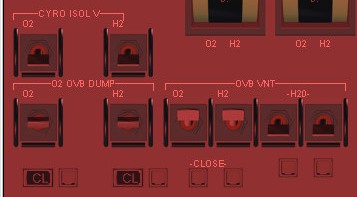
\includegraphics[width=0.5\hsize]{dragonfly_prsd_3.png}
\end{figure}

\noindent
OVB DUMP valves represent a high capacity (up to 450gr/sec) overboard vent valve, for quick discharge of reactants in case of emergency. OVB VENT valves are safety overpressure valves, that pneumatically open when reactant pressure exceed certain safety limits. In the case of O2, the safety overpressure valve will open at 1500 kPa and re-settle at 1450 kPa. For H2 the overpressure valve will open at 2500 kPa and re-settle at 2450kPa. For the H2O waste tank, the valve will open at 1000kPa and re-settle at 900kPa. The two H2O vent valves are non-propulsive, in that it will not affect the state vector of the ship. H2 and O2 valves, both DUMP and OVP will impact a small propulsive (-y axis) force when discharging. The high-capacity DUMP valves might take up to 10 second for opening/closing. A TB will indicate when the motor is operating. Additionally a OP/CL indicator will permanently indicate the respective position of the DUMP valve. Power for the high-capacity DUMP valve motor is also supplied by the battery and is not selectable by the crew.

\begin{figure}[H]
  \centering
  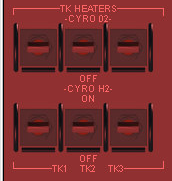
\includegraphics[width=0.25\hsize]{dragonfly_prsd_4.png}
\end{figure}

\noindent
TK HEATERS switches control electrical heaters that are located inside each cryogenic tank. Middle position (AUTO) will automatically turn the heaters on/off to maintain reactant pressure within operational limits.\\
When the heaters are at to AUTO position, the heaters will automatically be turned on for every tank that reaches a minimum operational pressure of 450kPa, for both O2 and H2 tanks, then turned off when the pressure reaches again 470kPa.As the tanks are depleted, the TK HEATERS should be turned to the off position to save electrical power and to prevent an overheating of the reactants. Basic FC operation is based on supercold reactants flowing throughout the FC stack for cooling purposes. Excessive heating of the reactants in order to maintain pressure means warmer reactants will enter the FC stack, which might lead to a FC overheating. An overheated FC will also produce warmer H2O as a byproduct, which in turn is used a a general coolant throughout the ship to maintain a thermal balance. A higher H2O temperature in the H2O tank means warmer water will flow through the coolant loops, leading to a large number of problems. Tank heaters are powered by their own DC bus, HTRS bus, linked to DC1.

\paragraph{Fuel Cells \& Battery}

\begin{figure}[H]
  \centering
  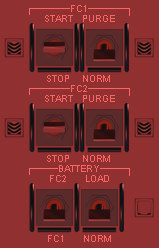
\includegraphics[width=0.25\hsize]{dragonfly_fc.png}
\end{figure}

\noindent
In normal operation mode, only one fuel cell (FC1) is active, running on reactants supplied by tanks 1 and 2. In case of exceeding power loads only, or as a back-up, FC2 might be started also. The two TB indicators monitor proper reactant flow into the respective FC. The TB will indicate white at nominal flow and barberpole if flow is less than nominal. The START/STOP switch controls power from the battery to the reactant pumps that direct O2 and H2 flow to the respective reaction plates inside the FC stack. The START switch must be held in the START momentary position for approximately 15-20 seconds until FC chemical reactions can supply enough power to the fuel pumps for self-sustainability, which is indicated by the two reactant TB turning white. The second PURGE/NORM switch will trigger the automatic purge sequence for the respective fuel cell. When set to purge, the pumps will direct as much as 900gr/min of reactants to the FC, for the high volume of reactants to clean the FC stack from diverse chemicals and residuals accumulated inside the FC stack during operation. FC purging can be confirmed by the high-flow indicated on the REACTANT FLOW indicator at the bottom-right part of the panel. Another indicator for FC purging is the FUEL PH monitor, located at the center of the panel. dPH should never exceed 1.5 for normal FC operation. As the dPH rises, FC performance is seriously affected and more reactants will be used to produce power until eventually the chain reaction will collapse. Because a small reactant flow rate will not clean any of the residuals and impurities inside the FC, running the FC at idle load will need a purge at smaller intervals than running the FC at normal power loads.\\
The resulting water from the FC chemical reaction will run to a H2O waste tank. Pressure in this tank can be monitored on the H2O WST TK indicator. The H2O OVP VENT should always be set to on during a FC purge sequence, to prevent damage from overpressuring the tank, or to prevent water from the tank, running up the piping back to the FC where it can kill the chemical reaction.\\
The last row of switches control battery reloading from power supplied by either FC1 or FC2. Note that the CB (circuit breaker) BT LOAD must be in the push (close) position (by default opened) for loading to occur. The TB indicator will show barberpole if power is being sent to the battery.

\paragraph{Electrical Power Distribution and Control (EPDC)}

\begin{figure}[H]
  \centering
  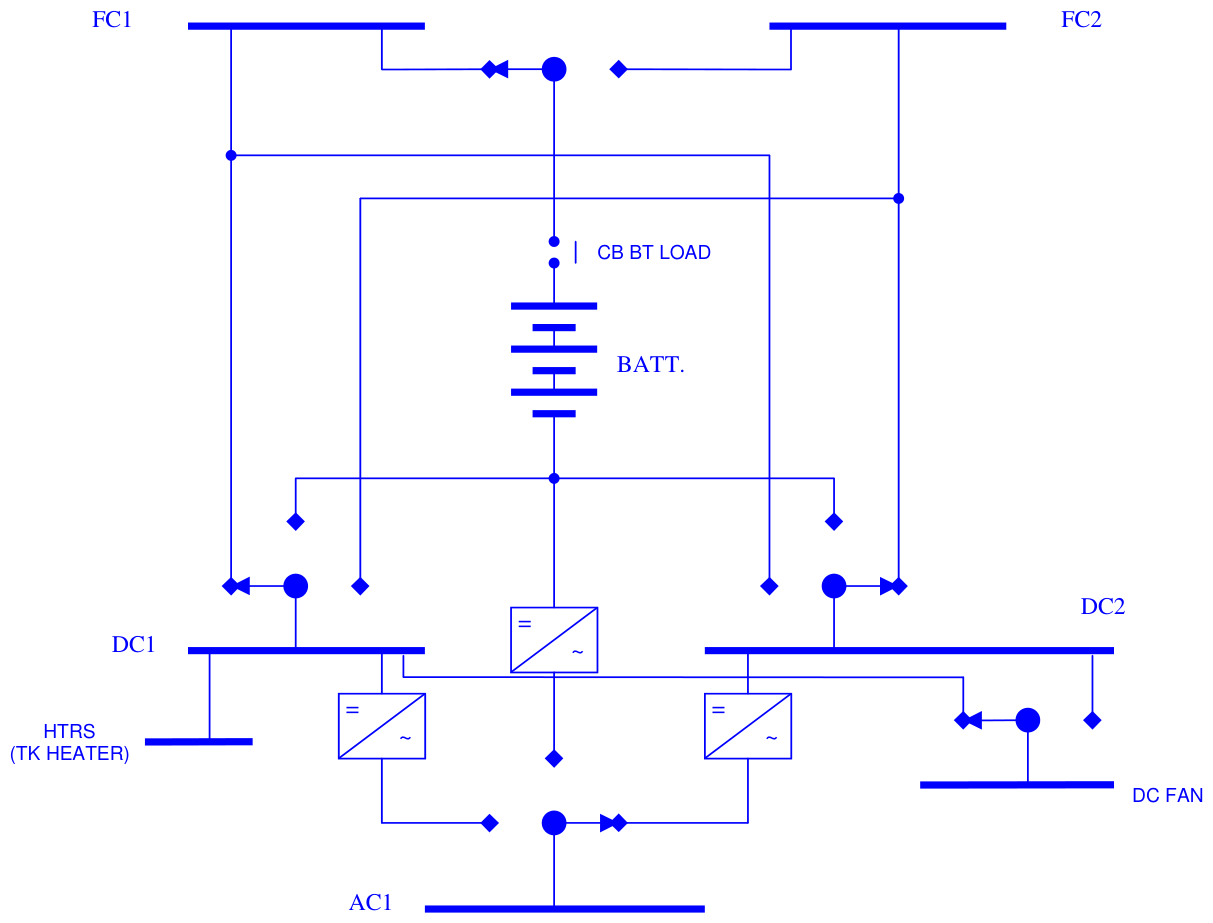
\includegraphics[width=\hsize]{dragonfly_diagram_epdc.png}
\end{figure}

\noindent
Electrical power inside the ship is provided trough two main Direct Current busses (DC1 and DC2) and one main Alternative Current bus (AC1). While most essential equipment is connected to DC1, it is possible to route power to these equipments using the back-up DC2 in case of a problem with DC1. AC power, trough AC1, is needed for radar antennas operations and radar antennas electrical pitch and yaw motors.

\begin{figure}[H]
  \centering
  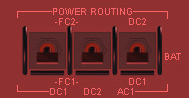
\includegraphics[width=0.25\hsize]{dragonfly_epdc_1.png}
\end{figure}

\noindent
The three POWER ROUTING switches are used to direct DC and AC loads to respective FCs or battery. From left to right, setting whether

\begin{itemize}
\item DC1 bus is linked to FC1 (down), the battery (middle) or FC2 (up)
\item DC2 bus is linked to FC2 (down), the battery (middle) or FC2 (up)
\item AC1 bus is linked to the DC1 bus (down), directly to the battery (middle) or to the DC2 bus (up)
\end{itemize}

\noindent
Note that the AC1 bus cannot be directly tied to a FC cell, as power must be converted by a static inverter into AC current. These static inverters exist only for DC1, DC2 and battery. Amperage and volts of the respective busses, battery and fuel cells can be monitored by the indicators located just above these switches.

\begin{figure}[H]
  \centering
  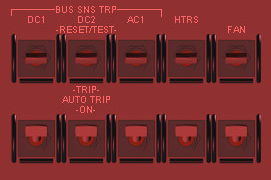
\includegraphics[width=0.35\hsize]{dragonfly_epdc_2.png}
\end{figure}

\noindent
Once linked to a power source, the respective DC and AC busses need to be re-mounted (turned on) for them to provide power. The respective CB (circuit breakers) need to be positioned in the pushed (close) position and the respective BUS SNS TRP switch must be brought to the momentary -RESET/TEST- position. If there is a problem within the bus, pressing this switch will cause an automatic disconnect of the bus from the power source, indicated by the respective CB popping back to the open position.

\begin{figure}[H]
  \centering
  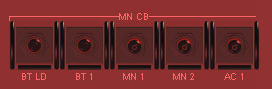
\includegraphics[width=0.35\hsize]{dragonfly_epdc_3.png}
\end{figure}

\noindent
CB indicators are located in the upper-right part of the panel. If the voltage and amperage are within operating limits, the CB indicator will remain in the pushed position and power will be routed trough that respective bus.\\
Pressing the same switch to its momentary -TRIP- position will automatically trip the respective bus.\\
NOTE. A bus should never be set to -TRIP - position, under normal circumstances, if connected to a FC load, much like an electrical instrument should not be instantly unplugged. Rather, that bus should be switched to battery or a non started FC and wait for the AUTO TRIP to automatically and safely shut down the respective bus.\\
The second row of switches (AUTO TRIP) if set to ON will automatically trip the respective bus if an out-of-limits situation occurs, such as low or high voltage, preventing equipment damage. The AUTO TRIP switch must be in it's ON position during a bus re-start to ensure a safe auto-shutdown of the bus.

\paragraph{Caution and Warning}

\begin{figure}[H]
  \centering
  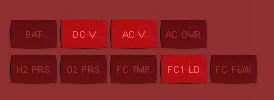
\includegraphics[width=0.5\hsize]{dragonfly_cw.png}
\end{figure}

Caution and warning displays on the electrical panel are located on the lower-left side. They present the crew with non-critical out-of-limits situations, making it easier to identify a problem.\\
The respective C/W will trigger under the following circumstances:

\begin{itemize}
\item BAT - Battery load. Less than 10kWh left in the battery, or battery overcharged.
\item DC V - Direct Current Voltage. One of the main DC busses (DC1 or DC2) has a voltage higher than 30 volts or lower than 27 volts.
\item AC V - Alternative Current Voltage. The main AC bus (AC1) has a voltage that exceeds 38 V or lower than 35 V
\item AV OVC - AC bus Overload. More than 100 A of load onto AC1
\item H2 PRS / O2 PRS - Cryogenic pressure is less than 200 kPa
\item FC TMP - FC 1 or 2 temp stack is larger than 350 K
\item FC1 LD - Fuel Cell 1 Load. Fuel cell 1 is either overloaded (> 200 A) or under-loaded (< 20 A)
\item FC FLW - Fuel Cell Flow. Reactant flow inside FC1 or FC2 is larger than the nominal 7.5 kg/h
\end{itemize}


\paragraph{EPS Procedures \& Checklists}
A. Normal operation switch positions:
%\begin{table}[H]
	%\centering
	\begin{longtable}{ p{\textwidth} }
	O2 TK1 ISOL VLV - OPEN\\
	O2 TK2 ISOL VLV - OPEN\\
	O2 TK3 ISOL VLV - CLOSE\\
	O2 XFEED 1 - OPEN\\
	O2 XFEED 2 - OPEN\\
	O2 REAC VLV FC1 - OPEN\\
	O2 REAC VLV FC2 - OPEN\\
	FC1 PURGE - NORM\\
	FC2 PURGE - NORM\\
	BAT LOAD - FC1, NORM\\
	H2 TK1 ISOL VLV - OPEN\\
	H2 TK2 ISOL VLV - OPEN\\
	H2 TK3 ISOL VLV - CLOSE\\
	H2 XFEED 1 - OPEN\\
	H2 XFEED 2 - OPEN\\
	H2 REAC VLV FC1 - OPEN\\
	H2 REAC VLV FC2 - OPEN\\
	TK HEATERS - ALL AUTO\\
	O2 ISOL VLV - OPEN\\
	H2 ISOL VLV - OPEN\\
	O2 OVB DUMP - CL\\
	H2 OVB DUMP - CL\\
	O2 OVP VENT - CL\\
	H2 OVP VENT - CL\\
	H2O OVP VENT - CL BOTH\\
	BUS SNS TRP AUTO TRIP - ALL ON\\
	\\
	CB BT LD - OPEN\\
	CB - ALL OTHER CLOSED\\
	\\
	POWER ROUTING\\
	\quad DC1 - FC1\\
	\quad DC2 - FC2\\
	\quad AC1 - DC2\\
	\end{longtable}
%\end{table}

\noindent
B. FC1 START:
%\begin{table}[H]
	%\centering
	\begin{longtable}{ p{\textwidth} }
	O2 TK1 ISOL VLV - OPEN\\
	H2 TK1 ISOL VLV - OPEN\\
	O2 REAC VLV FC1 - OPEN\\
	H2 REAC VLV FC1 - OPEN\\
	FC1 PURGE - NORM\\
	H2O OVP VENT - CL BOTH\\
	BAT LOAD - NORM\\
	FC1 START - HELD UNTIL TB TURN WHITE\\
	H2O OVP VENT - OP BOTH
	\end{longtable}
%\end{table}

\noindent
C. FC2 START (OPTIONAL)
%\begin{table}[H]
	%\centering
	\begin{longtable}{ p{\textwidth} }
	O2 TK1 ISOL VLV - OPEN\\
	O2 TK2 ISOL VLV - OPEN\\
	H2 TK1 ISOL VLV - OPEN\\
	H2 TK2 ISOL VLV - OPEN\\
	O2 XFEED 1 - OPEN\\
	O2 XFEED 2 - OPEN\\
	H2 XFEED 1 - OPEN\\
	H2 XFEED 2 - OPEN\\
	O2 REAC VLV FC2 - OPEN\\
	H2 REAC VLV FC2 - OPEN\\
	FC2 PURGE - NORM\\
	H2O OVP VENT - CL BOTH\\
	BAT LOAD - NORM\\
	FC2 START - HELD UNTIL TB TURN WHITE\\
	H2O OVP VENT - OP BOTH
	\end{longtable}
%\end{table}

\noindent
C. DC1 START
%\begin{table}[H]
	%\centering
	\begin{longtable}{ p{\textwidth} }
	POWER ROUTING DC1 - FC1 / FC2 / BAT - as req.'\\
	CB MN1 - PUSH CLOSED\\
	BUS SNS TRP AUTO TRIP DC1 - ON\\
	BUS SNS TRP DC1 - RESET / TEST
	\end{longtable}
%\end{table}

\noindent
D. DC2 START
%\begin{table}[H]
	%\centering
	\begin{longtable}{ p{\textwidth} }
	POWER ROUTING DC2 - FC1 / FC2 / BAT - as req.'\\
	CB MN2 - PUSH CLOSED\\
	BUS SNS TRP AUTO TRIP DC2 - ON\\
	BUS SNS TRP DC2 - RESET / TEST
	\end{longtable}
%\end{table}

\noindent
D. AC1 START
%\begin{table}[H]
	%\centering
	\begin{longtable}{ p{\textwidth} }
	POWER ROUTING AC1 - DC1 / DC2 / BAT - as req.'\\
	CB AC1 - PUSH CLOSED\\
	BUS SNS TRP AUTO TRIP AC1 - ON\\
	BUS SNS TRP AC1 - RESET / TEST
	\end{longtable}
%\end{table}

\noindent
E. HTRS / FAN BUS START
%\begin{table}[H]
	%\centering
	\begin{longtable}{ p{\textwidth} }
	CB HTRS - PUSH CLOSED\\
	CB FAN - PUSH CLOSED\\
	BUS SNS TRP AUTO TRIP HTRS - ON\\
	BUS SNS TRP HTRS - RESET / TEST\\
	BUS SNS TRP AUTO TRIP FAN - ON\\
	BUS SNS TRP FAN - RESET / TEST
	\end{longtable}
%\end{table}

\noindent
F. EPS START - UP
%\begin{table}[H]
	%\centering
	\begin{longtable}{ p{\textwidth} }
	POWER ROUTING DC1 - BAT\\
	POWER ROUTING AC1 - BAT\\
	C.DC1 START\\
	D.AC1 START\\
	CB BT LD - CLOSE\\
	BAT LOAD - FC2, LOAD\\
	B.FC1 START\\
	BAT LOAD - FC1, LOAD\\
	POWER ROUTING DC1 - FC1\\
	POWER ROUTING AC1 - DC1\\
	E. HTRS / FAN BUS START\\
	-WHEN BATTERY IS RECHARGED:\\
	\quad BAT LOAD - FC1, NORM\\
	\quad CB BT LD - OPEN
	\end{longtable}
%\end{table}

\noindent
G. EPS POWER-DOWN
%\begin{table}[H]
	%\centering
	\begin{longtable}{ p{\textwidth} }
	POWER ROUTING AC1 - DC1\\
	POWER ROUTING DC2 - BAT\\
	POWER ROUTING DC1 - BAT\\
	FC1 PURGE - NORM\\
	FC2 PURGE - NORM\\
	FC1 START - STOP\\
	FC2 START - STOP\\
	O2 TK ISOL VLV - ALL CLOSE (3)\\
	H2 TK ISOL VLV - ALL CLOSE (3)\\
	O2 ISOL VLV - CLOSE\\
	H2 ISOL VLV - CLOSE\\
	H2O OVP VENT - OPEN BOTH\\
	BUS SNS TRIP FAN - TRIP\\
	BUS SNS TRIP HTRS - TRIP\\
	BUS SNS TRIP AC1 - TRIP\\
	BUS SNS TRIP DC2 - TRIP\\
	BUS SNS TRIP DC1 - TRIP\\
	BUS SNS TRP AUTO TRIP - ALL OFF (5)
	\end{longtable}
%\end{table}

\noindent
H. FC PURGE
%\begin{table}[H]
	%\centering
	\begin{longtable}{ p{\textwidth} }
	H2O OVP VENT - OPEN BOTH\\
	O2 ISOL VLV - CLOSE\\
	H2 ISOL VLV - CLOSE\\
	POWER ROUTING - NO LOAD ON FC\\
	FC (1 / 2) PURGE - PURGE\\
	WAIT 0.3 < dPH < 0.7\\
	FC (1 / 2) PURGE - NORM\\
	POWER ROUTING - as req.'\\
	O2 ISOL VLV - as req.'\\
	H2 ISOL VLV - as req.'\\
	H2O OVP VENT - as req.'
	\end{longtable}
%\end{table}


\subsubsection{Environmental Control And Life Support System (ECLSS)}

\begin{figure}[H]
  \centering
  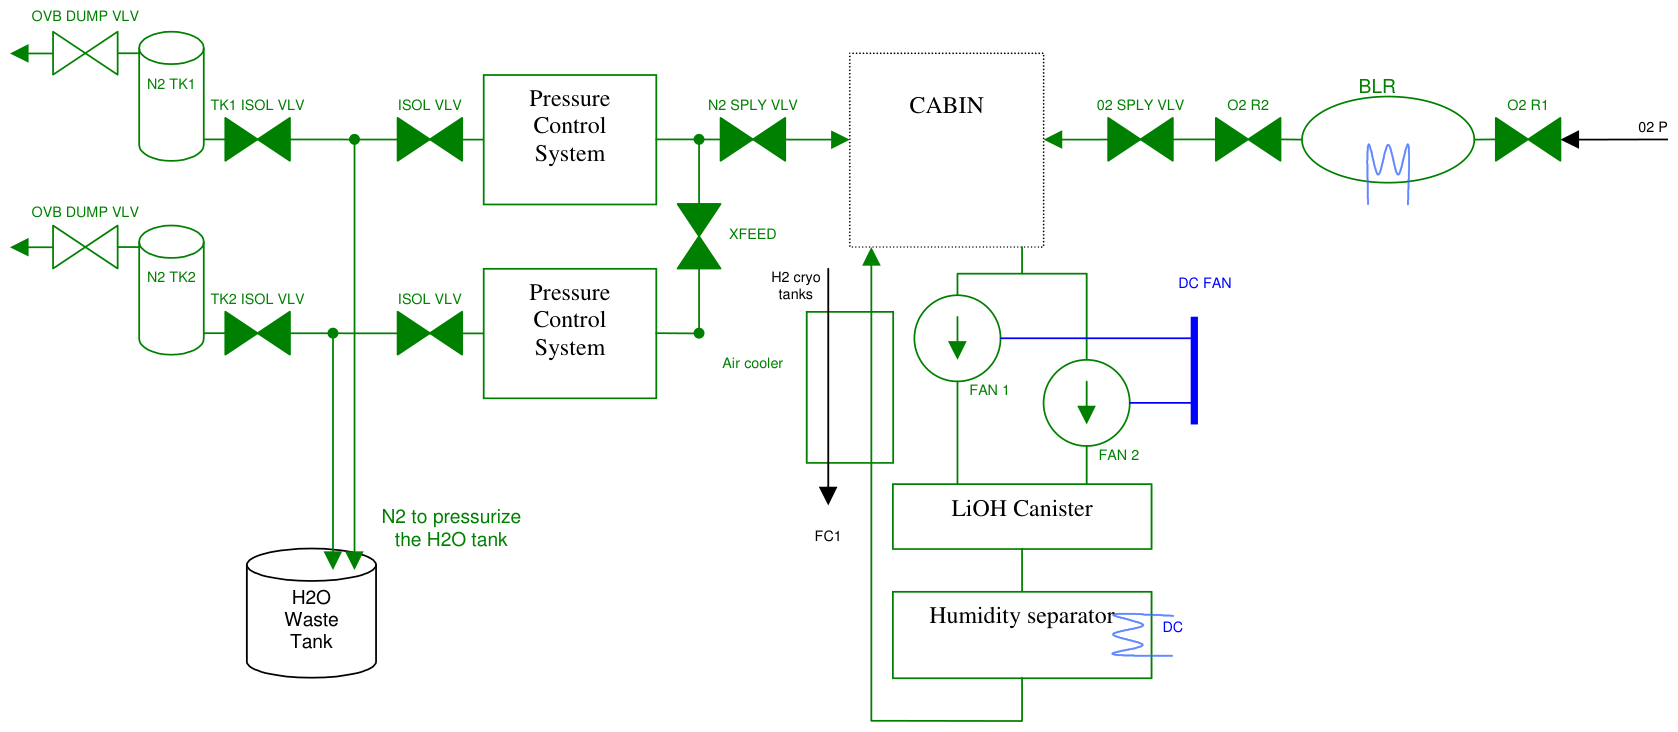
\includegraphics[width=\hsize]{dragonfly_diagram_eclss.png}
\end{figure}

\paragraph{Description}
The ECLSS maintains the spacecraft's thermal stability and provides a pressurized, habitable environment for the crew and onboard avionics. The ECLSS also manages the storage and disposal of water and crew waste. ECLSS is functionally divided into three systems:

\begin{itemize}
\item \textbf{Pressure control system}, which maintains the crew compartment at 103kPa with a breathable mixture of oxygen and nitrogen. Nitrogen is also used to pressurize the supply and wastewater tanks.
\item \textbf{Atmospheric revitalization system}, which uses air circulation and water coolant loops to remove heat, control humidity, and clean and purify cabin air.
\item \textbf{Active thermal control system}, (not implemented) which consists of two Freon loops that collect waste heat from orbiter systems and transfer the heat overboard, either trough radiators or ammonia boilers.
\end{itemize}

\noindent
As Dragonfly has not yet been equipped with active thermal control systems, most cooling and heating operations are done by passive control systems, whereas supercold cryogenic reactants are heated prior to entering the FC stack, thus cooling electrical equipment. The same is done with the wastewater, which is circulated throughout the vessel. As the water in the wastewater tank overheats, any boiling excess will be vented trough two non-propulsive vent valves. The only unbalanced thermal reaction is that of the FC, which, in the absence of active cooling equipment will overheat within 5-8 hours. The only cooling possibility for a FC is either shutting down (alternatively using FC1 / FC2) or purging.

\paragraph{Pressure control system}
The pressure control system normally pressurizes the crew cabin to 103 $\pm$ 10 kPa. It maintains the cabin at an average 70-percent nitrogen (27 kg) and 30-percent oxygen (9 kg) mixture that closely resembles the atmosphere at sea level on Earth. The system also provides the cabin atmosphere necessary to cool cabin-air-cooled equipment. Oxygen partial pressure is maintained automatically between 20 and 23 kPa, with sufficient nitrogen pressure of 78.3 kPa added to achieve the cabin total pressure of 103 $\pm$ 10 kPa. Positive and negative pressure relief valves protect the structural integrity of the cabin from over- and under-pressurization respectively. The pressure control system nitrogen is also used to pressurize the supply and wastewater tanks.

\begin{figure}[H]
  \centering
  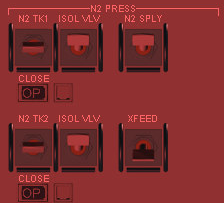
\includegraphics[width=0.35\hsize]{dragonfly_pcs_1.png}
\end{figure}

\noindent
Nitrogen is stored into two, identical, 3-liter tanks, serviced at a temperature of 288 K, that contain up to 20kg of N2 each. The provided nitrogen is enough to re-pressurize the cabin and docking hatch for up to 6 docking hatch re-pressurizations (EVAs). The two N2 TK1 and N2 TK2 switches, located on panel O1 (main ECLSS panel), control isolation valves to each of the two N2 tanks. When closed, N2 from that tank is not provided to either the pressure control system or as pressurizer for the wastewater-cooling loop. A second set of ISOL VLV control N2 flow from the tanks to the pressure control system. Note that N2 will continue to pressurize the wastewater tank, even with both of the ISOL VLV closed if any of the N2 TK valves are open.\\
The N2 SPLY switch will close the N2 from the pressure control system to be vented into the cabin, though N2 from the tanks, might continue to flow, either as pressurizer for the wastewater tanks, either to the over-pressure vent valves. N2 pressure is regulated at the N2 SPLY valve to a nominal pressure of 78-80kPa. The XFEED switched must be in its open position for tank 2 to provide N2 pressurization to the cabin. During normal operations only N2 tank 1 will be used for cabin pressurization and N2 tank 2 for wastewater cooling loop pressurization. A set of 2 (one for each tank) high-capacity N2 OVB DUMP valves will quickly discharge over-pressurized N2 from the N2 pressure control system.\\
Though the N2 tanks have no heaters to raise tank pressure, it is possible for excess heat from the wastewater cooling loop to transfer to the N2, thus overheating and over-pressurizing the N2 tanks. To avoid damage to the tanks, the two valves can be used to quickly discharge the overheated N2 and bring the tank pressure to a safer value.

\begin{figure}[H]
  \centering
  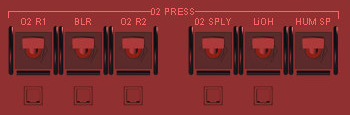
\includegraphics[width=0.5\hsize]{dragonfly_pcs_2.png}
\end{figure}

\noindent
Oxygen from the power reactant storage and distribution system (cryogenic oxygen supply system) is routed to the pressure control oxygen system, first to a pressure regulator (O2 R1) that reduces oxygen pressure to a lower 280-290 kPa. At this pressure an electrical boiling plate (BLR) can transform the cryogenic oxygen to its gaseous form by heating it to a service temperature of 295 K (22°C). The pressure gas from the boiler plate is then passed trough a second pressure regulator (O2 R2) that releases oxygen into the O2 pressure control system at 23-25 kPa and at an ambient temperature of 22°C. The same O2 SPLY valve as for N2, controls O2 discharge into the cabin circuit. Note that the boiler plate that heats oxygen from cryogenic to room temperature is powered not by the battery because of the rather large power consumption of the boiling plate. Instead, DC1 is used . Without DC power on the DC1 bus, the boiling plate will not be functional and no gaseous oxygen can be produces. Monitor the R1 TEMP R2 indicators to get a readout of the boiling plate functionality. Temperature for the R1 regulator, usually around the serviced 170 K is the temperature directly from the Cyro O2 PRSD manifold. Temperature of the second pressure regulator must be around 295 K which, at the serviced pressure of 1atm renders the oxygen to it's gaseous form. If the two temperatures are identical,the boiling plate is either unpowered, has been shut down or is damaged. At the cryogenic temperature of 170 K oxygen will remain in it's liquid form and will not be discarded into cabin atmosphere. Monitor the O2 FLOW indicator to get a reading of the amount of oxygen passing through the oxygen revitalization system.

\paragraph{Atmospheric revitalization system}

\begin{figure}[H]
  \centering
  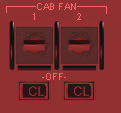
\includegraphics[width=0.2\hsize]{dragonfly_ars_1.png}
\end{figure}

\noindent
Two electrical fans provide the continuous air circulation needed in the cabin. Air from the cabin is directed into an air revitalization circuit, whereas CO2 is removed by LiOH canisters and humidity is controlled by a DC-powered humidity separator. Both fans function on an independent bus (DC FAN) that can be connected to either DC1 or DC2 main busses, or directly to the battery. From the LiOH and HUM SP the air piping then interleaves with cryogenic H2 passing from the H2 cryo tanks to FC1, thus cooling the air to a lower 22-25 C before returning it to the cabin. Before actually reaching the cabin the air is mixed with oxygen provided by R2 regulator, bringing fresh oxygen from the PRSD supply, if the R2 pressure valve switch is open.

\begin{figure}[H]
  \centering
  \includegraphics[width=0.5\hsize]{dragonfly_ars_2.png}
\end{figure}

\noindent
Most of the cabin air properties can be monitored on the top indicators on panel O1. O2 partial pressure, N2 partial pressure, CO2 partial pressure and total ambient pressure. Left indicators show cabin atmosphere status, while right indicators show docking hatch atm. status.

\begin{figure}[H]
  \centering
  \includegraphics[width=0.4\hsize]{dragonfly_ars_3.png}
\end{figure}

\noindent
Ambient temperature can also be monitored on this part of the panel. Ambient delta Pressure / delta Temperature can also be monitored to indicate eventual cabin leaks or depressurizations. A third indicator monitors the pressure difference between cabin air and atmospheric rev. system. A 0 delta pressure indicates an improper functioning of the two circulating fans, and that air is not circulated.

\paragraph{ECLSS Procedures \& Checklists}
A. Normal operation switch positions:

%\begin{table}[H]
	%\centering
	\begin{longtable}{ p{\textwidth} }
	N2 TK1 - OPEN\\
	N2 TK2 - OPEN\\
	N2 PRESS ISOL VLS - BOTH OPEN\\
	N2 PRESS XFEED - CLOSED\\
	N2 SPLY - OPEN\\
	N2 OVB VENT - BOTH CLOSED\\
	\\
	O2 PRESS R2 - CLOSED\\
	O2 PRESS BLR - OPEN\\
	O2 PRESS R1 - OPEN\\
	O2 SPLY -OPEN\\
	O2 LiOH - OPEN\\
	O2 HUM SP - OPEN\\
	\\
	CAB FAN 1, 2 - OP
	\end{longtable}
%\end{table}


\subsubsection{Communications}
TODO

\subsubsection{Radar And Docking Systems}
\paragraph{Description}
Being designed as a space tug, Dragonfly's primary mission is space components retrieval and handling, which will necessitate a large amount of docking operations. A large part of Dragonfly's systems, therefore, have been designed as to facilitate and automate docking operations. It features a Vicinity Awareness System (VAWS), two Doppler range and range-rate radar antennas, a visual docking sensor and two NAV radios.


\paragraph{Vicinity Awareness System (VAWS)}
VAWS provides the pilot with the situation awareness of the spacecrafts / spaceparts around his ship. It is composed by a number of 8 optical pairs of emitters/receptors positioned throughout the ship that give the VAWS a total operational range of 360° / 360° around the ship. Each of the 8 optical emmiters have a maximal optical resolution of ~0.11°, and are capable to detect (at max. range of 500m) objects as large as 1m.

\begin{figure}[H]
  \centering
  \includegraphics[width=0.4\hsize]{dragonfly_vaws.png}
\end{figure}

\noindent
The VAWS display consists of two radar projections, a top-down view on the left display and a right-left view on the right display. Both displays together can provide the user with a 3D description of the vessel parts around his craft.\\
Range can be selected in 50m increments up to the maximum range of 500m. The lower button on the left (VS) allows cycling trough all the detected signals. Pitch and azimuth bearings for the selected signal will be provided to the two Doppler range antennas for more accurate positional data. Antenna azimuth bearing is also displayed on the left display (top-down) as a dark-green 30° signal band.\\
Each of the two displays provides 4 light-green bands of 15°, marking the left/right, up/down, front/back areas where RCS firing could cause damage to proximity vessels. Use of RCS when a signal is detected in the light-green areas should be used very carefully, as to avoid RCS firing towards the signal. Note that most OVB dump valves and over-pressure valves are located as to fire on the +z axis (right). Special care must be taken that no signal enters the right-bound green stripe if danger of a overboard vent exists.


\paragraph{Doppler range and range-rate antennas}
The Dragonfly is equipped with a pair of long-range Doppler antennas capable of accurate measurements (0.01m/sec) of signal velocities. One antenna is mounted on the upper dome of the crew habitat, and one on the bottom, each one covering it's hemisphere. Each antenna has a movement capability of +/- 150° in yaw, for a total azimuth coverage of 300°, with a blackband of 60 deg in the rear of the vessel; and a total 75° pitch, with a blackband cone of 15 deg at the upper and lower poles of the vessel. Control for the antennas is located on panel R1.

\begin{figure}[H]
  \centering
  \includegraphics[width=0.2\hsize]{dragonfly_antenna_1.png}
\end{figure}

\noindent
There are two switches allowing movement control for each antenna. Y//R(L) and P//U(D) switches for yaw respectively pitch of the antenna dish. A third switch controls the antennas major operation mode. CNT (center) is used for parking the antennas at it's 0° pitch / 150° yaw position when the Doppler antennas are not used. Middle position sets the antennas in manual mode, where position can be controlled by the two upper switches. The third AQ\&TRK (Acquire and Track) mode will automatically direct the antennas to the yaw/pitch bearings of the signal selected in the VAWS.

\begin{figure}[H]
  \centering
  \includegraphics[width=0.4\hsize]{dragonfly_antenna_2.png}
\end{figure}

\noindent
Each of the antennae positions are indicated on the ANT YAW / ANT PITCH indicators. A third indicator (SGN) indicates signal strength on the Doppler antenna. Note that a minimum signal of 85\% is needed for the Doppler to accurately compute range and range-rate values.

\begin{figure}[H]
  \centering
  \includegraphics[width=0.4\hsize]{dragonfly_antenna_3.png}
\end{figure}

\noindent
On the front panel, data from the Doppler signal is interpreted and displayed to the user in an understandable and useful form. RADAR DIST - total distance to signal RADAR CLRS - closure rate, total relative velocity between Dragonfly and the signal on the bottom row, the relative velocity is split on each of the Dragonfly's three axes, respectively: lateral velocity (left-right), vertical velocity (up-down), forward velocity (front-back).\\
A RAD SGN (radar signal) TB indicator will indicate barber-pole when signal from the Doppler exists. All range and range-rate indicated when RAD SGN indicates white, are false or non-reliable at best.

\subsubsection{Front Panel Instruments}
\paragraph{Reaction Control System (RCS) modes}
The diferent available RCS modes can be controlled by the switches located in the lower/left part of the front panel.

\begin{figure}[H]
  \centering
  \includegraphics[width=0.4\hsize]{dragonfly_rcs.png}
\end{figure}

\noindent
Selectable RCS modes are:

\begin{itemize}
\item Linear / Rotation / Disabled
\item Normal / Vernier
\item Normal / Pulse / Rate
\item Kill Rot
\end{itemize}

\noindent
%TODO chech "by 1/10th" vs "to 1/10th"
The first switch in the left selects either linear or rotational major modes of the RCS. The second and third switch in the row select the RCS minor operational modes. Any combination of the settings can be used.\\
VERN minor mode will reduce thruster capacity by 1/10$^{th}$.\\
When PULSE minor rate is selected the RCS will fire short bursts (0.02 seconds) of thrust for each thrust command. The joystick controller will have to be re-centered until another command can be issued. For keyboard commands, the key must be released until another command is accepted.\\
When RATE minor mode is selected, each thrusting command will add 10\% of thrust (or 1\% if Vernier) to the respective thruster group. The joystick must be recentered, or the keyboard key released, until a new command is accepted. For example striking \keystroke{8}$_{Num}$ 3 times in \textit{linear non-vernier} mode, will engage the 'up' linear thrusters at 30\% of their capacity. Striking \keystroke{8}$_{Num}$ 6 times in \textit{rotational vernier} mode will engage the "pitch up" rotational thrusters at 6\% of their capacity. At any time hitting the reverse command (\keystroke{2}$_{Num}$ in this case) will close the RCS valves completely, regardless of their power setting.\\
The fourth CB controls the automatic rotational rate nullifier, ie. the KillRot. Note that this function is only available when major mode \textit{rotational, non-vernier, normal rate} is selected. Hitting \keystroke{5}$_{Num}$ at any other time will not engage the killrot command. Hitting the KILLROT CB on the front panel however will temporarily switch to major mode \textit{rotational, non-vernier, normal rate} then engage the killrot command. After the killrot program has completed, the previous RCS settings are restored.

\paragraph{Docking port management}
Because of the large number of docking operations, it is very important for a Dragonfly pilot to properly understand the management of Docking ports, which is provided by the instruments located at the center of the front panel.

\begin{figure}[H]
  \centering
  \includegraphics[width=0.3\hsize]{dragonfly_dock.png}
\end{figure}

\noindent
"Docking Sensor Input" allows the pilot to select which docking port is to be used as a \textit{source} by the Dock MFD.\\
For selecting the \textit{target} docking port, use normal Orbiter operations: either tune to the appropriate NAV frequency, or use the visual docking camera. The two buttons "VESSEL" and "PORT" will cycle trough all the vessels currently docked to the Dragonfly, respectively through all the docking ports of that vessel. "LOCAL PORT 0" is indicated when Dragonfly's own docking port is selected. Note that the RELASE DOCK switch (located just above) will undock the currently selected source docking port, and not necessarily Dragonfly's own docking port. This makes it possible for the pilot to trigger remote undocks for all the vessels currently docked together.\\
"CG Balance Offset" instructs the RCS system, as to where the center of gravity of the docked vessels is located. The RCS computer will then appropriately trigger the responsible thruster valves in such a manner as to produce only linear or rotational momentum, depending on the major RCS mode set. This is very important, as it allows the RCS to function properly even with large masses docked in front of the ship.

\paragraph{ADI ball}
The ADI ball is responsible with providing the 3D orientation of the vessel to the pilot. It is composed of a 6-degrees of freedom sphere, with unwinding engines (meaning it can rotate indefinitely in each direction). The ADI sphere, when powered (by main bus DC1), will maintain a fixed orientation in space, thus providing heading, pitch and roll indications of the current position of the ship.

\begin{figure}[H]
  \centering
  \includegraphics[width=0.5\hsize]{dragonfly_adi.png}
\end{figure}

\noindent
The ADI sphere is marked with concentric parallel rings at +30, +60, -30 and -60 degrees of pitch, with thin longitudinal marks for every 10° of yaw and thick longitudinal marks for every 30° of yaw. All numbers indicated on the sphere are 10's of degrees.\\
The ADI ball can provide attitude data in three modes, with respect to three different systems of reference, each selectable by the left-most switch located just to the right of the ADI sphere:

\begin{itemize}
\item HOR(izon) mode provides heading, pitch and roll information with respect to the local horizon.\\
Heading of 0 is calibrated as the geographical north. Pitch and roll are determined from the local horizontal plane. Heading information is local geographical azimuth.
\item GDC(guidange) mode provides yaw, pitch and roll information that is stored in Dragonfly's navigational computed. One of two guidance modes can be chosen from the middle switch:

\begin{itemize}
\item ECL(iptic) mode considers the vernal point at MJD 2000 as the 0° heading (+x axis), the ecliptic north as the +90° pitch (+y axis) and their cross-product as the 90° heading (+z axis). Yaw information is therefore ecliptic hour of ascension, pitch information is ecliptic declination. This mode can be mainly used for platform alignment and star tracking.
\item ORB(ital) mode considers the orbital prograde point as the 0° heading (+x axis), the normal to the orbital plane as the +90° pitch (+y axis) and their cross-product as the 90° heading (+z axis). This mode can be mainly used for orbital operations.
\end{itemize}

\item REF(erence) will display attitude data with respect to a pre-set system of axes. When the third switch (right-most) is put to the momentarily position MARK, the current ship attitude is stored. REF mode will further indicate the changes in pitch, roll and yaw since the last stored attitude.
\end{itemize}

\noindent
The motors driving the ADI sphere operate with a maximum speed of 25°/sec. If rotational rates ever exceed the ADI operational limits, the TB indicator located on the upper-right corner will indicate an over-drive, meaning the ball has reached it's maximum operational speed. The information indicated by the sphere while the TB indicator is barberpole is not reliable.\\
The TB indicator will also turn barberpole when the sphere is being moved from one reference mode to another. This is normal.


\subsection{Space Shuttle Atlantis}
% TODO


\subsection{International Space Station (ISS)}
The International Space Station is a multinational scientific orbital platform in low Earth orbit (orbital altitude $\sim$420 km). It is composed of multiple modules that were assembled in orbit from 1998. It has been continuously occupied since 2000 and is expected to be in operation until 2030. Many of the assembly missions (with the exception of the Russian modules) and crew operation missions were flown by the Space Shuttle until its retirement in 2011, which makes the ISS a good mission target for your Shuttle flights. Docking the Space Shuttle manually at the ISS with its Orbital Docking System installed in the payload bay is a challenge even for experienced pilots.

\begin{figure}[H]
  \centering
  \includegraphics[width=0.75\hsize]{iss.jpg}
  \caption{3D model and textures: Project Alpha by Andrew Farnaby}
\end{figure}

\noindent
The ISS is equipped with multiple docking ports. In Orbiter, they are outfitted with IDS (Instrument Docking System) transmitters to feed the onboard docking instruments. The default IDS frequencies are listed in the table.

%\begin{table}[H]
	%\centering
	\begin{longtable}{ |p{0.1\textwidth}|p{0.15\textwidth}| }
	\hline\rule{0pt}{2ex}
	Port 1 & 137.40  MHz\\
	\hline\rule{0pt}{2ex}
	Port 2 & 137.30  MHz\\
	\hline\rule{0pt}{2ex}
	Port 3 & 137.20  MHz\\
	\hline\rule{0pt}{2ex}
	Port 4 & 137.10  MHz\\
	\hline\rule{0pt}{2ex}
	Port 5 & 137.00  MHz\\
	\hline
	\end{longtable}
%\end{table}

\noindent
In addition, a transponder (XPDR) for long-range tracking at frequency 131.30 MHz is equipped.

\begin{figure}[H]
  \centering
  \includegraphics[width=0.75\hsize]{iss_dock.png}
  \caption{Effect of RCS command input on linear/rotational alignment cues in Docking MFD for Shuttle with docking adapter installed in cargo bay.}
\end{figure}


\subsection{Space Station Mir}
Mir was a Soviet (later Russian) modular space station in low Earth orbit ($\sim$360 km altitude) between 1986 and 2001. It was assembled in stages, with modules delivered to orbit mostly by Proton rockets. It was the largest man-made object in orbit before being surpassed by the ISS. It was continuously inhabited and still holds the record for longest human spaceflight. At the end of it service life it was de-orbited and burnt up in the atmosphere, with remaining fragments falling into the South Pacific Ocean.\\

\begin{figure}[H]
  \centering
  \includegraphics[width=0.75\hsize]{mir.jpg}
  \caption{Mir model and textures by Jason Benson.}
\end{figure}

\noindent
In Orbiter, Mir is still in orbit and can be used for rendezvous and docking manoeuvres. Unlike its real-life counterpart, it is orbiting in the plane of the ecliptic, which makes it a good staging platform for translunar and interplanetary missions.\\
Mir supports 3 docking ports, which in Orbiter are equipped with IDS with transmitting at the frequencies listed in the table. It also has a long-range transponder (XPDR) at 132.10 MHz.

%\begin{table}[H]
	%\centering
	\begin{longtable}{ |p{0.1\textwidth}|p{0.15\textwidth}| }
	\hline\rule{0pt}{2ex}
	Port 1 & 135.00  MHz\\
	\hline\rule{0pt}{2ex}
	Port 2 & 135.10  MHz\\
	\hline\rule{0pt}{2ex}
	Port 3 & 135.20  MHz\\
	\hline
	\end{longtable}
%\end{table}


\subsection{Lunar Wheel Station}
This is a large fictional space station in orbit around the Moon. It consists of a wheel, attached to a central hub with two spokes. The wheel has a diameter of 500 m and is spinning at a frequency of one cycle per 36 s, providing its occupants with a centrifugal acceleration of 7.6 m/s$^{2}$, or about 0.8 g, to mimic Earth's surface gravitational force.

\begin{figure}[H]
  \centering
  \includegraphics[width=0.75\hsize]{lunar_wheel.jpg}
  \caption{A Shuttle-A on final approach to the Lunar Wheel station. Wheel model and textures: Martin Schweiger.}
\end{figure}

\noindent
%TODO add section link
The main problem the station poses to an approaching spacecraft is the rotational alignment in preparation for docking. Docking with a rotating target is only possible along the rotation axis. The station has two docking ports in the central hub, with approach directions along the axis from either side. Before docking, the approaching vessel must synchronise its own rotation around its longitudinal axis with that of the station. This should happen as late as possible (within 10 m separation), because corrections in the lateral position become very difficult once the spacecraft is rotating. For docking procedures, see Chapter TODO.\\

\alertbox{Currently, Orbiter's docking alignment instrumentation works with rotating docking targets only if the ship's docking port is aligned with its longitudinal axis of rotation. This is the case for Shuttle-A and Dragonfly, but not for the Delta-glider. And should you somehow get the Space Shuttle into a lunar orbit, don't even try to dock at the Wheel.}

\noindent
\\
The Wheel station emits a transponder signal at frequency 132.70 MHz. The default IDS transmitter frequencies for the two docking ports are listed in the table.

%\begin{table}[H]
	%\centering
	\begin{longtable}{ |p{0.1\textwidth}|p{0.15\textwidth}| }
	\hline\rule{0pt}{2ex}
	Port 1 & 136.00  MHz\\
	\hline\rule{0pt}{2ex}
	Port 2 & 136.20  MHz\\
	\hline
	\end{longtable}
%\end{table}


\subsection{Hubble Space Telescope}
The Hubble Space Telescope (HST) was launched into low Earth orbit by Space Shuttle Discovery during mission STS-31 in 1990 and is still in operation as of 2022. Several on-orbit service missions have been carried out until the retirement of the Space Shuttle program, one of which was to install corrective optics to compensate for a shape error of the primary mirror which was discovered after the telescope had been launched.

\begin{figure}[H]
  \centering
  \includegraphics[width=0.75\hsize]{hst.jpg}
  \caption{HST model and textures by David Sundstrom.}
\end{figure}

\noindent
Hubble mainly operates in the visible frequency range (from near-infrared to ultraviolet). As a space-based telescope, it avoids image degradation from atmospheric effects, and during its long service life it provided images of unprecedented quality that significantly contributed to advance our understanding of the universe. Its observations range from solar system objects and events, such as the impact of comet Shoemaker-Levy on Jupiter, to deep-field images of the faintest and most distant objects yet observed in the visible band. Notable discoveries to which Hubble data contributed include the accelerated expansion of the universe, the prevalence of supermassive black holes in the centres of galaxies, detection of exosolar planets and evidence of star formation.\\
%TODO add section link
Orbiter provides several Space Shuttle\textbackslash HST missions for both deployment and recapture operations. For Shuttle payload manipulation, see Chapter TODO.\\
\\
\textbf{Vessel-specific key controls:}

%\begin{table}[H]
	%\centering
	\begin{longtable}{ |p{0.2\textwidth}|p{0.7\textwidth}| }
	\hline\rule{0pt}{2ex}
	\textbf{Shortcut} & \textbf{Action}\\
	\hline\rule{0pt}{2ex}
	1 & Deploy/retract high-gain antennae\\
	\hline\rule{0pt}{2ex}
	2 & Open/close telescope tube hatch\\
	\hline\rule{0pt}{2ex}
	3 & Deploy/fold solar arrays\\
	\hline
	\end{longtable}
%\end{table}


\subsection{LDEF Satellite}
The Long Duration Exposure Facility (LDEF) was an orbital platform designed to provide experimental data on the effect of space environment on materials, biological samples and operational procedures. It was delivered to orbit by Space Shuttle Challenger in 1984 (mission STS-41 C). It was intended to be recaptured and returned to Earth a year later, but due to delays in the aftermath of the Challenger accident, was stranded in space for six years and eventually recovered from its decaying orbit on January 11, 1990 by Columbia (STS-32), two months before it would have burnt up in the atmosphere.

\begin{figure}[H]
  \centering
  \includegraphics[width=0.75\hsize]{ldef.jpg}
  \caption{LDEF mesh by Don Gallagher.}
\end{figure}

\noindent
The LDEF makes a good object for Shuttle deployment and retrieval missions in Orbiter. Scenario folder Satellites and Probes\textbackslash LDEF contains missions for LDEF operations.


\end{document}
